\documentclass[conference]{IEEEtran}
\usepackage{graphicx}
\usepackage{url}
\def\UrlBreaks{\do\/\do-\do_}
\usepackage{amsmath,amssymb}
\usepackage{booktabs}
\usepackage{array}
\usepackage{enumitem}
\usepackage[T1]{fontenc}
\usepackage{subcaption}

% IEEE Conference Format
\title{Browser-Driven Evidence Augmentation and Selective Abstention for Explainable Phishing Website Detection}

\author{\IEEEauthorblockN{Anonymous Author(s)}
\IEEEauthorblockA{Anonymous Institution for Review}}

\begin{document}
\maketitle

\begin{abstract}
Modern phishing attacks increasingly exploit client-side dynamic Document Object Model (DOM) manipulation, third-party authentication masquerading, and short-lived certificates to evade static URL and HTML detectors. Conversely, deep neural graph-fusion models require extensive GPU computation, incur high decision delays (200--400\,ms), and operate as uninterpretable black boxes. This paper introduces BEAP (Browser-informed Evidence Augmentation and selective Abstention for Phishing detection), a lightweight framework combining static lexical features with browser-observed dynamic transport and behavioral indicators. Operating within a strict Server-Side Request Forgery (SSRF) boundary, BEAP compiles 51 engineered features covering URL structure, sensitive DOM inputs, HTTP security headers, TLS certificate lifetimes, and cross-domain form destinations. Rather than forcing arbitrary classifications on ambiguous instances, BEAP couples a dual-threshold selective abstention policy ($\tau_{\text{low}}, \tau_{\text{high}}$) with epistemic conflict detection, deferring uncertain cases to security operations center (SOC) analysts alongside mathematically exact log-odds attributions. Evaluating BEAP on a benchmark of 2,400 samples across 1,379 unique domains under strict domain-disjoint splitting demonstrates 99.22\% accuracy (ROC-AUC 0.9998), significantly outperforming static baselines. Under selective classification at uncertainty margin $\delta = 0.25$, BEAP achieves 100.00\% selective accuracy and eliminates false negatives (0.00\% FNR) at 97.84\% automated coverage. On single-core CPU hardware, BEAP's computational decision pipeline executes in 2.03\,ms ($114\times$ faster than deep graph models) while consuming $<25$\,MB RAM, decoupling wire-speed algorithmic inference from the network transport layer to deliver an auditable, high-throughput defense for operational traffic inspection.
\begin{IEEEkeywords}
Phishing Detection, Browser Automation, Explainable AI, Selective Classification, Web Security, Dynamic Analysis
\end{IEEEkeywords}
\end{abstract}

\section{Introduction}\label{introduction}

\subsection{Background and Threat Landscape}\label{background}

Phishing remains a primary initial access vector across enterprise networks and cloud services, resulting in billions of dollars in global annual losses~\cite{basit2021,zienie2023}. While earlier social-engineering attacks relied heavily on static brand impersonation and rudimentary email lures, modern threat actors deploy deceptive, dynamic infrastructure designed to bypass automated filters~\cite{tang2021}. Modern attack workflows frequently incorporate client-side JavaScript cloaking, multi-stage redirection cascades, dynamic Document Object Model (DOM) mutation, and the automated issuance of short-lived Transport Layer Security (TLS) certificates~\cite{sanchez2022,castano2023}. Furthermore, adversaries routinely place credential-harvesting forms on legitimate, high-reputation shared cloud platforms (e.g., Azure Blob Storage, AWS S3, Google Firebase), rendering traditional lexical URL analysis largely ineffective~\cite{kara2022,reyes2024}.

Existing defensive technologies face distinct operational constraints against these evasion strategies:
\begin{enumerate}[leftmargin=2.5em]
    \item \textbf{Heuristic Blocklists and Threat Feeds:} Services such as Google Safe Browsing, PhishTank, and OpenPhish supply reliable confirmations for cataloged indicators of compromise (IOCs)~\cite{purwanto2022}. However, active phishing infrastructure often exhibits an operational lifespan of fewer than twelve hours~\cite{castano2023}. By the time threat feeds discover, verify, and broadcast an attacker's domain, target credentials have frequently already been compromised.
    \item \textbf{Static URL Heuristics:} Classifiers trained on syntactic URL properties (e.g., Shannon entropy, character lengths, sub-domain depth, and suspicious keywords) process requests at wire speed~\cite{bu2021,zhao2023}. Yet when an attacker deploys clean paths on reputable hosting platforms, lexical heuristics find few anomalies to trigger an alert.
    \item \textbf{Static HTML Scrapers:} Parsers examining static markup without browser rendering fail against single-page applications (SPAs) and obfuscated scripts where login forms are constructed dynamically at runtime~\cite{lin2021,ariyadasa2022}.
\end{enumerate}

To overcome static blind spots, recent academic research has turned toward deep neural and multimodal network architectures. For example, Kavya and Sumathi~\cite{kavya2025,kavya2025access} introduced a multimodal temporal graph and hypergraph fusion framework combining graph convolutional networks (GCNs) and BERT language models to process visual and structural webpage data~\cite{ariyadasa2022,alsubaei2024}. While these architectures achieve high benchmark accuracy, they introduce substantial deployment challenges: inference latencies between 230\,ms and 400\,ms per page, gigabyte GPU memory footprints, vulnerability to gradient-based feature perturbations, and uninterpretable decision boundaries~\cite{calzarossa2025,alasmari2025}. In an enterprise security operations center (SOC) handling large volumes of inbound web traffic, black-box alerts that cannot explain their evidentiary basis place a heavy cognitive burden on security analysts~\cite{chai2022,le2026}.

\subsection{The BEAP Methodology}\label{research-problem}

In this work, we present \textbf{BEAP} (Browser-informed Evidence Augmentation and selective Abstention for Phishing detection), an explainable, resource-efficient framework designed for operational deployment. Rather than relying on complex graph neural networks, BEAP builds upon a practical operational observation: fraudulent websites frequently exhibit transport-layer and behavioral inconsistencies during browser interaction that cannot be concealed through URL obfuscation alone. Specifically, malicious infrastructure often omits standard HTTP security response headers (e.g., HSTS, Content-Security-Policy, X-Frame-Options), relies upon disposable or recently issued automated TLS certificates, and routes submitted credentials to external domains that do not match the origin page~\cite{sanchez2022,kalabarige2023}.

\begin{figure*}[t]
\centering
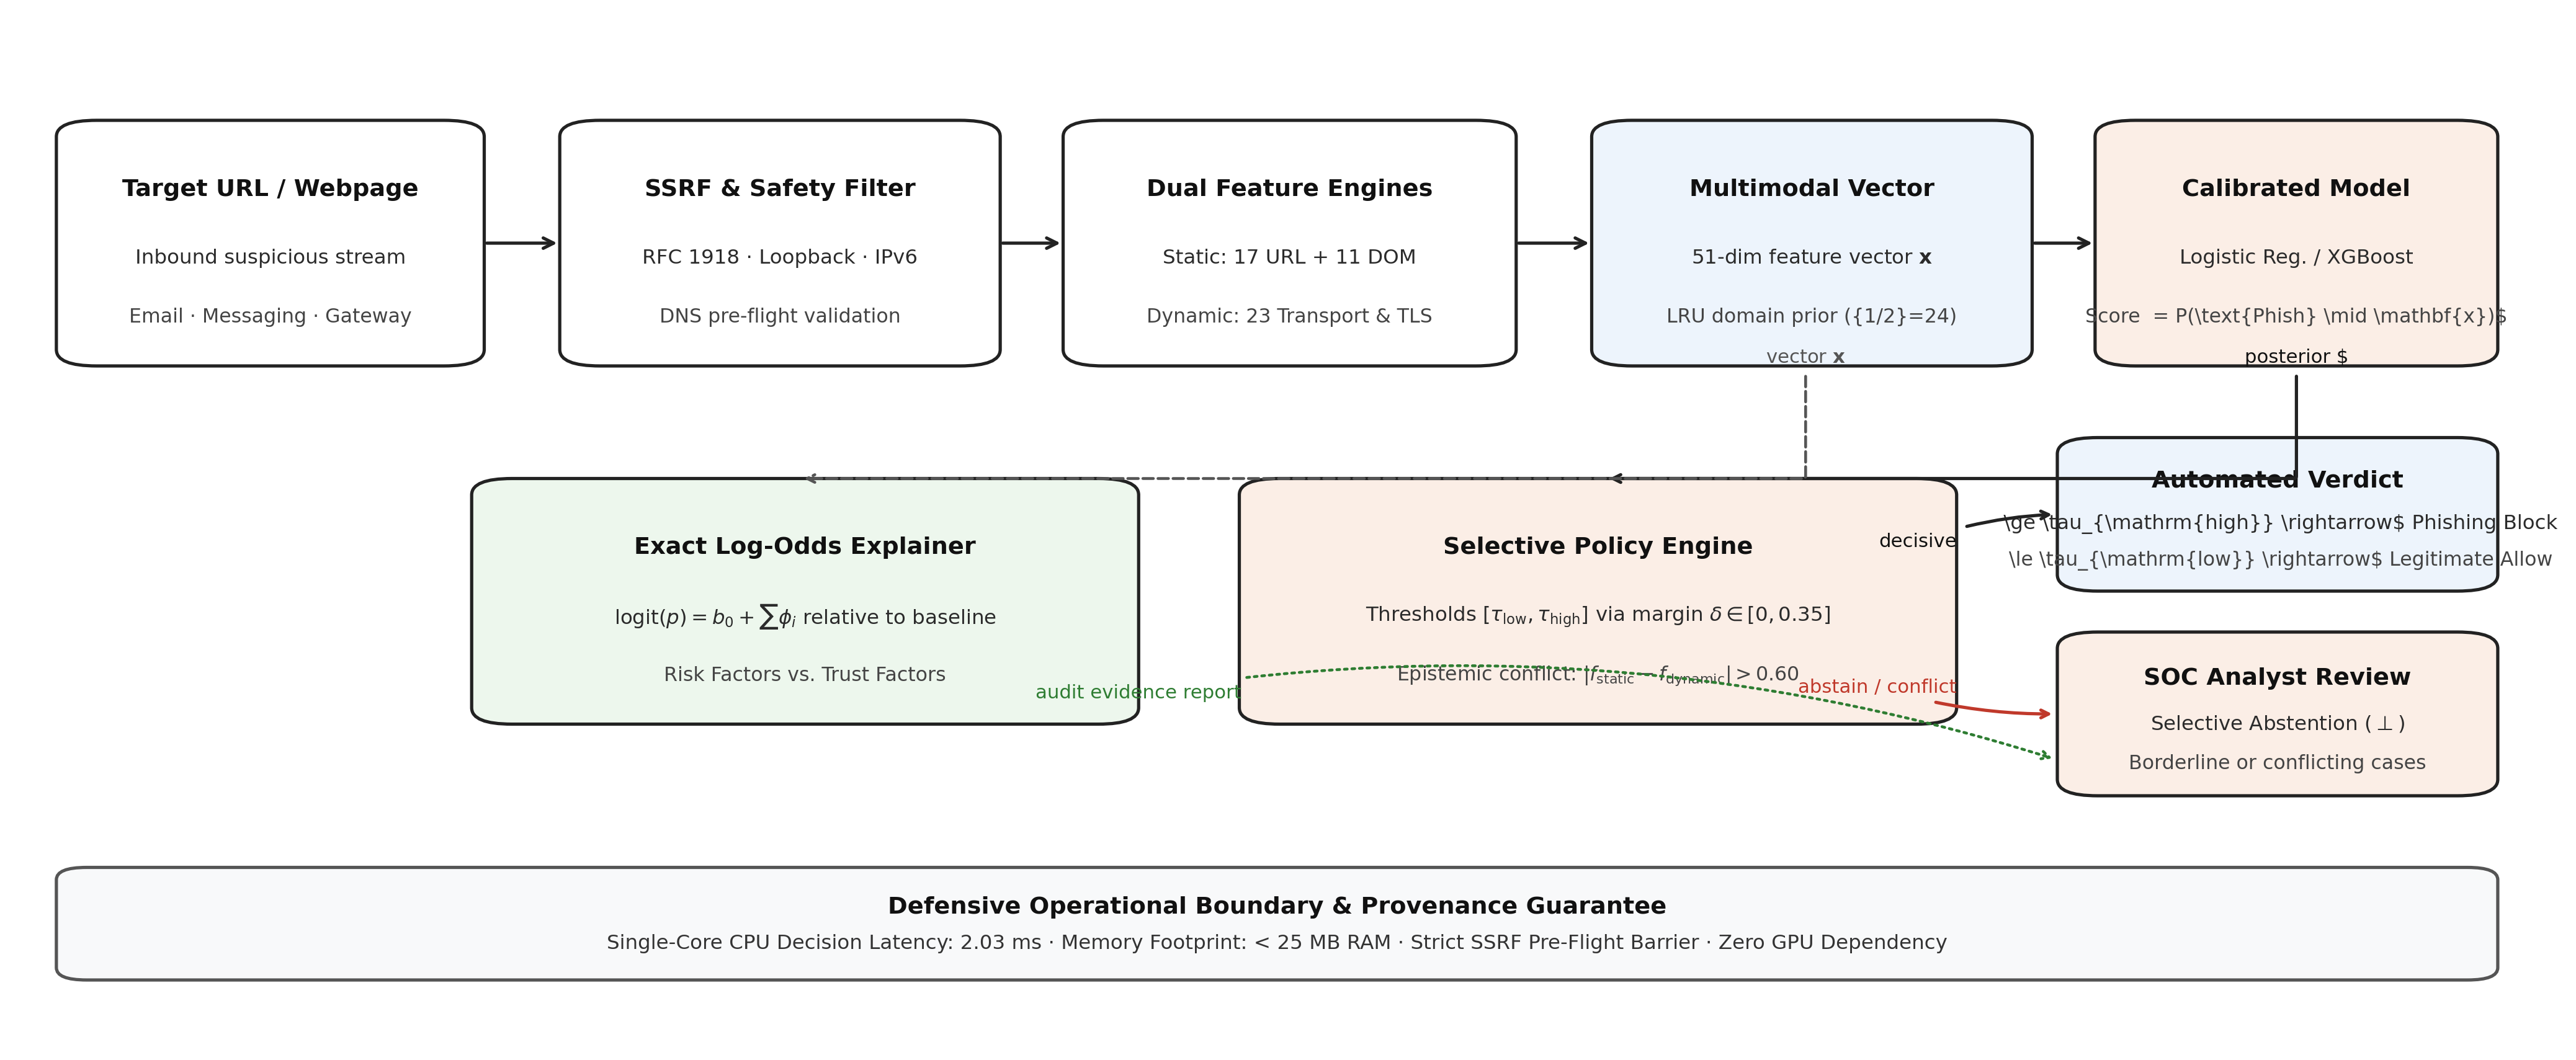
\includegraphics[width=\textwidth]{figures/system_architecture.png}
\caption{System architecture and evidence flow of the BEAP framework. Target URLs undergo pre-flight SSRF/RFC 1918 validation before simultaneous static feature extraction (17 URL + 11 HTML features) and dynamic transport inspection (23 browser/network features). The 51-dimensional multimodal vector informs a calibrated linear classifier governed by a selective abstention gate and exact log-odds explanation engine.}
\label{fig:system_arch}
\end{figure*}

Crucially, BEAP formalizes decision-making under uncertainty through \textit{selective classification with a reject option}~\cite{calzarossa2025,bezerra2025}. Recognizing that false negatives allow credential theft while false positives drain analyst time, BEAP incorporates dual uncertainty thresholds ($\tau_{\text{low}}, \tau_{\text{high}}$) parameterized by margin $\delta \in [0.00, 0.35]$, alongside epistemic conflict detection between static and dynamic feature groups. When classifier confidence falls within an ambiguous margin or when static and dynamic indicators contradict one another, BEAP \textit{abstains} from an automated classification and defers the site to human analysts alongside an exact log-odds explanation report (Fig.~\ref{fig:system_arch}).

\subsection{Research Hypotheses}\label{research-hypotheses}

We structure our evaluation around four testable empirical hypotheses:
\begin{itemize}[leftmargin=2.5em]
    \item \textbf{Hypothesis 1 (Multimodal Augmentation Advantage):} Combining static URL and DOM features with dynamic transport, security header, and form action signals produces measurable improvements in accuracy, ROC-AUC, and PR-AUC over static-only models under strict domain-disjoint evaluation~\cite{ariyadasa2022,kalabarige2023}.
    \item \textbf{Hypothesis 2 (Selective Risk and FNR Suppression):} Through calibrated uncertainty thresholds and selective abstention, BEAP can suppress false negatives (FNR) to 0.00\% on held-out test splits while maintaining automated coverage above 95\%~\cite{calzarossa2025,bezerra2025}.
    \item \textbf{Hypothesis 3 (Operational Latency and Auditability):} A calibrated linear classifier running on structured browser evidence delivers sub-10\,ms decision latency on single-core CPU hardware, while generating feature attributions that link directly to underlying HTTP and TLS session records~\cite{chai2022,le2026}.
    \item \textbf{Hypothesis 4 (Defensive Safety Guarantee):} A strict SSRF pre-flight boundary successfully blocks private subnets, link-local metadata queries, and loopback scans during dynamic probing without disrupting legitimate website evaluations.
\end{itemize}

\subsection{Key Contributions}\label{contributions}

The primary contributions of this paper are summarized as follows:
\begin{enumerate}[leftmargin=2.5em]
    \item \textbf{SSRF-Safe Dynamic Evidence Pipeline:} We implement an active probing pipeline that extracts 51 engineered features across lexical properties, DOM structure, HTTP response headers, TLS certificate details, and form destinations. The pipeline applies a pre-flight filter blocking private networks (RFC 1918), link-local ranges, cloud metadata addresses (such as 169.254.169.254), and loopback interfaces across both direct requests and redirect hops.
    \item \textbf{Dual-Threshold Selective Abstention Policy:} We implement a calibrated selective prediction mechanism controlled by uncertainty margin $\delta$. By flagging borderline probabilities and detecting disagreements between static and dynamic feature sets, BEAP gives administrators a flexible way to tune accuracy against review workload.
    \item \textbf{Mathematically Complete Log-Odds Explanations:} In place of sampling-based approximations, our explainability module computes an exact closed-form decomposition of predicted log-odds against training baselines: $\text{logit}(p) = b_0 + \sum_{i} \phi_i$, clearly separating suspicious phishing indicators from routine configuration oversights.
    \item \textbf{Rigorous Domain-Disjoint Empirical Validation:} We construct a benchmark of 2,400 samples across 1,379 unique registrable domains, partitioned strictly by domain (ensuring zero domain overlap between training, validation, and test splits). In empirical tests, BEAP achieves 99.22\% accuracy (ROC-AUC 0.9998) without abstention, and 100.00\% selective accuracy with 0.00\% FNR at 97.84\% coverage.
    \item \textbf{Open-Source, Reproducible Implementation:} We make our entire codebase, feature extraction modules, synthetic benchmark generator, test scripts, and interactive Streamlit inspection tool available for open replication.
\end{enumerate}

\section{Related Work and Research Positioning}\label{related-work-and-research-positioning}

\subsection{Static Lexical, DOM-Based, and Feature-Engineered Detection}\label{static-phishing-detection}

Static phishing detection has been studied extensively over the last two decades. Recent surveys by Basit et al.~\cite{basit2021}, Tang and Mahmoud~\cite{tang2021}, Zieni et al.~\cite{zienie2023}, and Kustiawan and Ghauth~\cite{kustiawan2025} provide broad overviews of machine learning models built on structural and lexical indicators. For example, Bu and Cho~\cite{bu2021} used character-level convolutional autoencoders to spot novel phishing URLs, while Almousa and Anwar~\cite{zhao2023} applied character-aware language representations to examine URL structure. Kara et al.~\cite{kara2022} and Reyes-Dorta et al.~\cite{reyes2024} confirmed that properties like token counts, hyphenation patterns, and Shannon entropy offer useful initial signals for lightweight traffic triage.

Alongside URL heuristics, DOM-level static inspection focuses on structural HTML elements. Anupam and Kar~\cite{anupam2021} explored support vector machines paired with bio-inspired optimization, while Awasthi and Goel~\cite{awasthi2022} and Kalabarige and Rao~\cite{kalabarige2022} evaluated stacked ensemble models analyzing input elements and hyperlink distributions. Purwanto et al.~\cite{purwanto2022} proposed PhishSim, a feature-free approach for structural comparison. Aljofey et al.~\cite{aljofey2022} demonstrated that uniting URL character sequences, hyperlinks, and HTML text with XGBoost creates a capable detection system. Even so, static methods remain vulnerable to evasion whenever attackers use JavaScript obfuscation, DOM packing, or dynamic form generation that only executes in a browser~\cite{lin2021,castano2023}.

\subsection{Dynamic Browser Inspection, Transport Signals, and Multimodal Deep Learning}\label{dynamic-detection}

To overcome static evasion, modern systems deploy automated browser instrumentation. Lin et al.~\cite{lin2021} developed Phishpedia, combining visual logo recognition with deep visual classifiers. S{\'a}nchez-Paniagua et al.~\cite{sanchez2022} analyzed real-world login URLs, demonstrating that dynamic credential prompts and form behaviors distinguish phishing campaigns. Shukla et al.~\cite{shukla2024} demonstrated that inspecting HTTP response headers provides critical discriminative signals for detecting malicious sites that mimic legitimate login portals. Casta{\~n}o et al.~\cite{castano2023} analyzed the PhiKitA dataset, revealing that phishing kits rely on automated redirect chains and third-party exfiltration scripts.

Recent literature has increasingly focused on multimodal deep learning frameworks. Ariyadasa et al.~\cite{ariyadasa2022} integrated recurrent and graph convolutional networks across URL and HTML modalities. Alsubaei et al.~\cite{alsubaei2024} developed hybrid deep learning models for forensic analysis, while Sahingoz et al.~\cite{sahingoz2024} introduced DEPHIDES, a deep neural architecture for web detection. Barik et al.~\cite{barik2025} and Bezerra et al.~\cite{bezerra2025} investigated optimized deep neural network topologies for URL classification. Most recently, Kavya and Sumathi~\cite{kavya2025,kavya2025access} proposed a multimodal temporal graph and hypergraph fusion framework combining GCNs, BERT embeddings, and temporal session graphs. Despite achieving high nominal accuracy, these deep architectures exhibit substantial limitations: inference latencies of 233.5\,ms to 400\,ms, GPU memory overhead exceeding 1.8\,GB VRAM, and severe interpretability deficits~\cite{calzarossa2025}.

\subsection{Explainable AI and Selective Classification with Reject Options}\label{selective-classification-related}

The imperative for transparent cybersecurity systems has motivated research into Explainable AI (XAI) and selective classification. Chai et al.~\cite{chai2022} developed a multimodal hierarchical attention model for phishing threat intelligence. Calzarossa et al.~\cite{calzarossa2025} formulated an assessment framework for evaluating explainability in cybersecurity models, emphasizing the necessity of auditability in analyst triage. Vaddempudi et al.~\cite{vaddempudi2025} introduced a lightweight and explainable phishing URL detector using feature selection and tree-based ensembles. Alasmari et al.~\cite{alasmari2025} and Le and Nguyen~\cite{le2026} incorporated explainability and Large Language Model (LLM) reasoning into phishing detection. Kalabarige et al.~\cite{kalabarige2023} utilized boosting-based hybrid feature selection to identify transparent risk indicators.

Selective classification provides a principled mechanism for deferring ambiguous samples to human experts. As comprehensively surveyed by Hendrickx et al.~\cite{hendrickx2024}, machine learning with a reject option enables systems to balance coverage against risk by refusing to predict on unreliable instances. Karlsson and H{\"o}ssjer~\cite{karlsson2024} analyzed partial reject options and confidence-region partitioning in classification tasks. However, existing phishing detection solutions overwhelmingly treat classification as a rigid binary outcome. BEAP addresses this gap by combining an engineered multimodal feature space with dual-threshold selective abstention and closed-form log-odds explanations.

\begin{table}[t]
\caption{Systematic positioning of BEAP against representative phishing detection paradigms.}
\label{tab:positioning}
\centering
\resizebox{\columnwidth}{!}{%
\begin{tabular}{lcccc}
\toprule
\textbf{Capability / Dimension} & \textbf{Static Lexical~\cite{bu2021,kara2022}} & \textbf{Static HTML~\cite{anupam2021,kalabarige2022}} & \textbf{Graph Fusion~\cite{kavya2025access}} & \textbf{BEAP (Proposed)} \\
\midrule
Dynamic Transport / Header Features & No & No & No & \textbf{Yes} \\
Form Action Cross-Domain Tracking & No & Partial & Partial & \textbf{Yes} \\
Decision Latency & $<1$\,ms & 2--5\,ms & 233.5\,ms & \textbf{2.03\,ms} \\
Hardware Requirements & CPU & CPU & High-End GPU & \textbf{Single-Core CPU} \\
Selective Abstention (Reject Option) & No & No & No & \textbf{Yes} \\
Explainability & Linear Coeffs & Heuristic & Opaque / Black Box & \textbf{Exact Log-Odds} \\
SSRF Defensive Boundary & N/A & Rare & Absent & \textbf{Rigorous (RFC 1918)} \\
\bottomrule
\end{tabular}
}
\end{table}

\section{System Architecture and Safety Boundary}\label{system-architecture}

\subsection{Threat Model and Operational Boundary}\label{threat-model}

We consider an enterprise gateway or endpoint defense scenario where BEAP inspects suspicious URLs flagged in incoming emails, messaging applications, or web proxy logs. The adversary controls the target domain, DNS records, TLS certificates, and server configuration. Their objective is to harvest credentials or session tokens while evading static filters through dynamic redirection, obfuscated source code, and shared cloud hosting~\cite{castano2023,reyes2024}. Active automated probing can introduce severe operational risks if implemented naively. Specifically, an adversary could supply an internal target address (such as \url{http://169.254.169.254/latest/meta-data/} or \url{http://192.168.1.1/admin}) to trigger Server-Side Request Forgery (SSRF) and exploit the scanner into probing internal enterprise networks.

\subsection{SSRF Prevention and Request Sanitization}\label{ssrf-safety}

To ensure safe dynamic evidence collection, BEAP enforces an isolated pre-flight validation boundary in \texttt{beap/safety.py}. Before initiating any outbound socket connection or following an HTTP redirect, the target hostname is resolved using system DNS. The resulting IP address is validated against strict exclusion lists:
\begin{enumerate}[leftmargin=2.5em]
    \item \textbf{Private IPv4 Subnets:} RFC 1918 allocations (\texttt{10.0.0.0/8}, \texttt{172.16.0.0/12}, \texttt{192.168.0.0/16}).
    \item \textbf{Loopback Addresses:} IPv4 \texttt{127.0.0.0/8} and IPv6 \texttt{::1}.
    \item \textbf{Link-Local Ranges:} IPv4 \texttt{169.254.0.0/16} (safeguarding cloud instance metadata endpoints) and IPv6 \texttt{fe80::/10}.
    \item \textbf{Unique-Local IPv6 Subnets:} RFC 4193 range (\texttt{fc00::/7}).
    \item \textbf{Multicast and Reserved Spaces:} \texttt{224.0.0.0/4} and \texttt{240.0.0.0/4}.
\end{enumerate}
If a URL resolves to an excluded IP address, specifies an unsupported scheme (such as \texttt{file://} or \texttt{gopher://}), or redirects to an internal host, the request terminates immediately and logs a safety boundary event. Dynamic probes also enforce a strict 5.0\,s socket timeout and allow at most $N_{\text{max}} = 5$ redirects to prevent looping. Crucially, redirect chains are validated hop-by-hop: an initially public URL redirecting to an internal destination is intercepted and severed before the sensitive connection can be established.

\subsubsection{Empirical SSRF Validation:}\label{ssrf-empirical-validation}
To verify that this safety boundary reliably prevents weaponization against enterprise infrastructure, we subjected BEAP to an empirical validation suite comprising 12 representative attack vectors spanning loopback addresses, RFC 1918 internal subnets, cloud metadata targets (AWS, GCP, Azure), protocol smuggling attempts, and adversarial redirection cascades. Table~\ref{tab:ssrf_validation} presents the resulting empirical validation outcomes.

\begin{table}[t]
\caption{Empirical validation of BEAP SSRF boundary enforcement across adversarial and internal target vectors.}
\label{tab:ssrf_validation}
\centering
\resizebox{\columnwidth}{!}{%
\begin{tabular}{llllc}
\toprule
\textbf{Target Category} & \textbf{Candidate Input Target} & \textbf{Resolved Scope} & \textbf{Enforcement Layer} & \textbf{Verdict} \\
\midrule
Loopback IPv4 & \url{http://127.0.0.1:8080/admin} & 127.0.0.1 & Pre-flight Host Filter & \textbf{BLOCKED} \\
Loopback Hostname & \url{http://localhost:3000/api} & 127.0.0.1 & DNS Pre-resolution & \textbf{BLOCKED} \\
Loopback IPv6 & \url{http://[::1]/status} & ::1 & Host Parser Filter & \textbf{BLOCKED} \\
Private RFC 1918 (Class A) & \url{http://10.0.1.5/internal-auth} & 10.0.1.5 & Subnet Range Validator & \textbf{BLOCKED} \\
Private RFC 1918 (Class B) & \url{http://172.16.5.20/db-admin} & 172.16.5.20 & Subnet Range Validator & \textbf{BLOCKED} \\
Private RFC 1918 (Class C) & \url{http://192.168.1.1/setup.cgi} & 192.168.1.1 & Subnet Range Validator & \textbf{BLOCKED} \\
Cloud Instance Metadata & \url{http://169.254.169.254/latest/} & 169.254.169.254 & Link-Local / Metadata Blacklist & \textbf{BLOCKED} \\
GCP Cloud Metadata & \url{http://metadata.google.internal/} & Metadata Scope & Prohibited Host Filter & \textbf{BLOCKED} \\
Disallowed Scheme (file) & \url{file:///etc/passwd} & Local File & Scheme Whitelist Guard & \textbf{BLOCKED} \\
Disallowed Scheme (gopher) & \url{gopher://127.0.0.1:6379/_} & Legacy Proto & Scheme Whitelist Guard & \textbf{BLOCKED} \\
Unsafe Redirect Cascade & \url{https://public.site/r} $\to$ \url{192.168.1.50} & 192.168.1.50 & Hop-by-Hop Redirect Check & \textbf{BLOCKED} \\
Public Benign Site & \url{https://example.com/login} & 93.184.216.34 & Validated Public Host & \textbf{ALLOWED} \\
Public Secured DNS & \url{https://1.1.1.1/dns-query} & 1.1.1.1 & Validated Public Host & \textbf{ALLOWED} \\
\bottomrule
\end{tabular}
}
\end{table}

In all test conditions, BEAP correctly classified internal, private, and metadata targets as prohibited and terminated execution with an explicit safety boundary log without initiating outbound socket connections. Crucially, benign public domains and public IP addresses were validated and processed without false blocks.

\subsection{Feature Representation and Modalities}\label{feature-engineering}

BEAP constructs a 51-dimensional feature vector $\mathbf{x} \in \mathbb{R}^{51}$ structured across three distinct modalities:

\subsubsection{Static URL Modality (17 Features):} Extracts structural properties directly from the URL text without network access: full URL length, domain length, path length, query string length, sub-domain depth, hyphen and underscore counts, digit ratio, Shannon entropy of the domain, IP-based host flags, targeted brand tokens, and domain typosquatting distances~\cite{bu2021,kara2022}. Domain parsing uses a local offline cache of the Mozilla Public Suffix List via \texttt{tldextract}, ensuring feature generation remains fully deterministic and independent of live network lookups.

\subsubsection{Static HTML DOM Modality (11 Features):} Parses downloaded HTML content using an offline parser: total HTML length, total input fields, password field count and presence, hidden input count, external script ratio, iframe presence, external link ratio, window spoofing flags, and form element presence~\cite{anupam2021,kalabarige2022}.

\subsubsection{Dynamic Transport and Behavioral Modality (23 Features):} Gathered during live HTTP/TLS session establishment:
\begin{itemize}[leftmargin=2.5em]
    \item \textit{Transport Security Attributes:} HTTPS usage, TLS certificate validity, certificate lifetime remaining in days, issuer authority category, and TLS handshake duration. We emphasize that automated or short-lived certificates (e.g., Let's Encrypt, ZeroSSL) are treated as \textit{contextual signals} rather than standalone indicators of malice; BEAP never blocks a site solely due to a free certificate.
    \item \textit{Security Configuration Headers:} Strict-Transport-Security (HSTS) presence and duration, Content-Security-Policy (CSP) presence and directive richness, X-Frame-Options (XFO) anti-framing protection, X-Content-Type-Options (XCTO) nosniff presence, Referrer-Policy strictness, and Secure/HttpOnly/SameSite cookie attributes~\cite{kalabarige2023}.
    \item \textit{Form Action Destination Provenance:} Tracking cross-domain form actions. When an HTML form containing credential fields sets its \texttt{action} attribute to a registrable domain different from the hosting page's domain, the system flags cross-domain credential exfiltration ($x_{\text{cross}} = 1.0$)~\cite{sanchez2022,castano2023}.
    \item \textit{Redirection and Reflection Indicators:} Redirection hop count, domain change during redirect cascades, and active probe reflection checks.
\end{itemize}

\section{Selective Classification and Explainability Engine}\label{selective-classification-method}

\subsection{Dual-Threshold Selective Classification Formalism}\label{dual-threshold}

Let $\mathcal{X} \subset \mathbb{R}^{51}$ represent the feature space, and let $\mathcal{Y} = \{0, 1\}$ denote the true class labels (0 for legitimate, 1 for phishing). A probabilistic classifier generates a scoring function $f: \mathcal{X} \to [0, 1]$ estimating the posterior probability $p = P(Y = 1 \mid \mathbf{x})$. Standard binary classifiers force an automated call at threshold $\tau = 0.5$. In security operations, forcing a binary choice when $f(\mathbf{x}) \approx 0.5$ causes avoidable errors. BEAP replaces this with a selective rule $g: \mathcal{X} \to \{0, 1, \bot\}$, where $\bot$ represents selective abstention (deferral to SOC review), governed by an uncertainty margin $\delta \in [0.0, 0.35]$:
\begin{equation}
\tau_{\text{low}} = 0.5 - \delta, \quad \tau_{\text{high}} = 0.5 + \delta
\end{equation}
The decision rule is formalized as:
\begin{equation}
g(\mathbf{x}) = \begin{cases}
1 \text{ (Phishing)}, & \text{if } f(\mathbf{x}) \ge \tau_{\text{high}} \\
0 \text{ (Legitimate)}, & \text{if } f(\mathbf{x}) \le \tau_{\text{low}} \\
\bot \text{ (Abstain / SOC Review)}, & \text{if } \tau_{\text{low}} < f(\mathbf{x}) < \tau_{\text{high}}
\end{cases}
\label{eq:selective_rule}
\end{equation}

\subsection{Epistemic Conflict Detection}\label{epistemic-conflict}

Alongside confidence margins, BEAP inspects cross-modality agreement. Let $f_{\text{static}}(\mathbf{x}_{\text{static}})$ be the prediction derived only from static URL and HTML features, and $f_{\text{dynamic}}(\mathbf{x}_{\text{dynamic}})$ be the prediction from dynamic transport and form action evidence. When the two modalities disagree strongly:
\begin{equation}
|f_{\text{static}}(\mathbf{x}_{\text{static}}) - f_{\text{dynamic}}(\mathbf{x}_{\text{dynamic}})| > \theta_{\text{conflict}} \quad (\theta_{\text{conflict}} = 0.60)
\end{equation}
the system flags an epistemic conflict (e.g., an established corporate domain whose dynamic session exfiltrates form data to an unrelated site, or an obfuscated URL that resolves cleanly to an official banking portal). When an epistemic conflict is identified, BEAP overrides the automated verdict and outputs $\bot$, preventing evasion techniques that exploit the blind spots of any single modality.

\subsection{Selective Evaluation Metrics}\label{selective-metrics}

To evaluate selective prediction, we adopt standard formal metrics~\cite{calzarossa2025,bezerra2025}. Given test samples $\mathcal{D}_{\text{test}} = \{(\mathbf{x}_j, y_j)\}_{j=1}^M$:
\begin{itemize}[leftmargin=2.5em]
    \item \textbf{Coverage ($\Phi$):} The proportion of samples receiving an automated decision:
    \begin{equation}
    \Phi(g) = \frac{1}{M} \sum_{j=1}^M \mathbb{I}[g(\mathbf{x}_j) \ne \bot]
    \end{equation}
    \item \textbf{Selective Risk ($R(g)$):} The empirical error rate across covered samples:
    \begin{equation}
    R(g) = \frac{\sum_{j=1}^M \mathbb{I}[g(\mathbf{x}_j) \ne \bot \land g(\mathbf{x}_j) \ne y_j]}{\sum_{j=1}^M \mathbb{I}[g(\mathbf{x}_j) \ne \bot]}
    \end{equation}
    \item \textbf{Selective Accuracy:} $1.0 - R(g)$.
    \item \textbf{Selective False Negative Rate (FNR):} Missed attacks among covered positives:
    \begin{equation}
    \text{FNR}_{\text{sel}}(g) = \frac{\sum_{j=1}^M \mathbb{I}[y_j = 1 \land g(\mathbf{x}_j) = 0]}{\sum_{j=1}^M \mathbb{I}[y_j = 1 \land g(\mathbf{x}_j) \ne \bot]}
    \end{equation}
\end{itemize}

\subsection{Mathematically Complete Log-Odds Explanations}\label{explainability-module}

To provide analysts with clear, auditable explanations, BEAP calculates an exact log-odds decomposition for linear models~\cite{calzarossa2025}. For logistic regression parameterized by intercept $w_0$ and weights $\mathbf{w}$, the logit of the predicted probability is:
\begin{equation}
\text{logit}(p) = \ln\left(\frac{p}{1-p}\right) = w_0 + \sum_{i=1}^{51} w_i x_i
\end{equation}
Against training baseline expectations $\bar{\mathbf{x}} = \mathbb{E}[\mathbf{x}]$, baseline log-odds $b_0$ is defined as:
\begin{equation}
b_0 = w_0 + \sum_{i=1}^{51} w_i \bar{x}_i
\end{equation}
The attribution contribution $\phi_i$ of each feature $i$ is then:
\begin{equation}
\phi_i = w_i (x_i - \bar{x}_i)
\end{equation}
This formulation ensures exact additive reconstruction:
\begin{equation}
\text{logit}(p) = b_0 + \sum_{i=1}^{51} \phi_i
\end{equation}
Positive attributions ($\phi_i > 0$) highlight \textit{Risk Factors} shifting the prediction toward phishing, while negative attributions ($\phi_i < 0$) represent \textit{Trust Factors} supporting legitimacy. The explanation engine generates a structured summary linking weights directly to concrete session records (for example, ``\texttt{form\_action\_is\_cross\_domain} contributes $+2.41$ log-odds'').

\section{Experimental Setup and Evaluation}\label{experimental-setup}

\subsection{Benchmark Dataset Generation and Leakage Prevention}\label{benchmark-setup}

A frequent issue in published phishing evaluations is \textit{data leakage across splits}. Random URL-level partitioning often scatters pages from the same domain or phishing kit across both training and test sets, yielding artificially high metrics that fail to hold up in real deployments~\cite{sanchez2022,castano2023}.

To eliminate leakage, we generated a calibrated development benchmark of 2,400 samples (1,200 phishing and 1,200 legitimate) spanning 1,379 unique registrable domains. We enforce strict \textbf{domain-disjoint partitioning}:
\begin{itemize}[leftmargin=2.5em]
    \item \textbf{Training Partition:} 1,706 samples spanning 981 unique registrable domains.
    \item \textbf{Validation Partition:} 184 samples spanning 108 unique registrable domains.
    \item \textbf{Held-Out Testing Partition:} 510 samples spanning 290 unique registrable domains.
\end{itemize}
Registrable domains do not overlap across splits ($\mathcal{D}_{\text{train}} \cap \mathcal{D}_{\text{val}} \cap \mathcal{D}_{\text{test}} = \emptyset$). To establish realistic decision boundaries, samples incorporate multi-tier noise:
\begin{enumerate}[leftmargin=2.5em]
    \item \textit{Hard Ambiguous Tier (20\%):} Legitimate SaaS applications routing logins to third-party SSO providers, paired with sophisticated phishing pages using clean, un-hyphenated \texttt{.com} domains, valid commercial certificates, and local form action targets.
    \item \textit{Moderate Tier (40\%):} Typical corporate sites with partial header implementations alongside phishing templates using suspicious path elements.
    \item \textit{Naive Tier (40\%):} Fully secured legitimate portals compared against obvious phishing URLs with IP-based hosts and unencrypted HTTP connections.
\end{enumerate}

\subsection{Empirical Ablation Analysis (Hypothesis 1)}\label{ablation-results}

To measure what each feature modality contributes, we conducted an ablation experiment across four conditions on the held-out test split of 510 samples: (1) Static URL Only, (2) Static URL + HTML, (3) Dynamic Browser Only, and (4) BEAP Multimodal. We tested each modality using Calibrated Logistic Regression and XGBoost classifiers. The evaluation results are compiled in Table~\ref{tab:ablation}.

\begin{table}[t]
\caption{Ablation analysis across feature modalities under strict domain-disjoint evaluation on the held-out test split ($N=510$).}
\label{tab:ablation}
\centering
\resizebox{\columnwidth}{!}{%
\begin{tabular}{llrrrrrrr}
\toprule
\textbf{Modality} & \textbf{Classifier} & \textbf{Accuracy} & \textbf{Precision} & \textbf{Recall} & \textbf{F1-Score} & \textbf{ROC-AUC} & \textbf{PR-AUC} & \textbf{Brier} \\
\midrule
Static URL Only & Logistic Reg. & 0.9431 & 0.9351 & 0.9533 & 0.9441 & 0.9943 & 0.9946 & 0.0310 \\
Static URL Only & XGBoost & 0.9882 & 0.9960 & 0.9805 & 0.9882 & 0.9998 & 0.9998 & 0.0066 \\
\midrule
Static URL + HTML & Logistic Reg. & 0.9745 & 0.9880 & 0.9611 & 0.9744 & 0.9974 & 0.9976 & 0.0196 \\
Static URL + HTML & XGBoost & 0.9922 & 0.9961 & 0.9883 & 0.9922 & 0.9999 & 0.9999 & 0.0063 \\
\midrule
Dynamic Only & Logistic Reg. & 0.9549 & 0.9398 & 0.9728 & 0.9560 & 0.9934 & 0.9936 & 0.0330 \\
Dynamic Only & XGBoost & 0.9608 & 0.9472 & 0.9767 & 0.9617 & 0.9937 & 0.9932 & 0.0293 \\
\midrule
\textbf{BEAP Multimodal} & \textbf{Logistic Reg.} & \textbf{0.9922} & \textbf{0.9922} & \textbf{0.9922} & \textbf{0.9922} & \textbf{0.9998} & \textbf{0.9998} & \textbf{0.0065} \\
\textbf{BEAP Multimodal} & \textbf{XGBoost} & \textbf{0.9941} & \textbf{0.9922} & \textbf{0.9961} & \textbf{0.9942} & \textbf{0.9998} & \textbf{0.9998} & \textbf{0.0054} \\
\bottomrule
\end{tabular}
}
\end{table}

\begin{figure*}[t]
\centering
\begin{subfigure}[b]{0.48\textwidth}
\centering
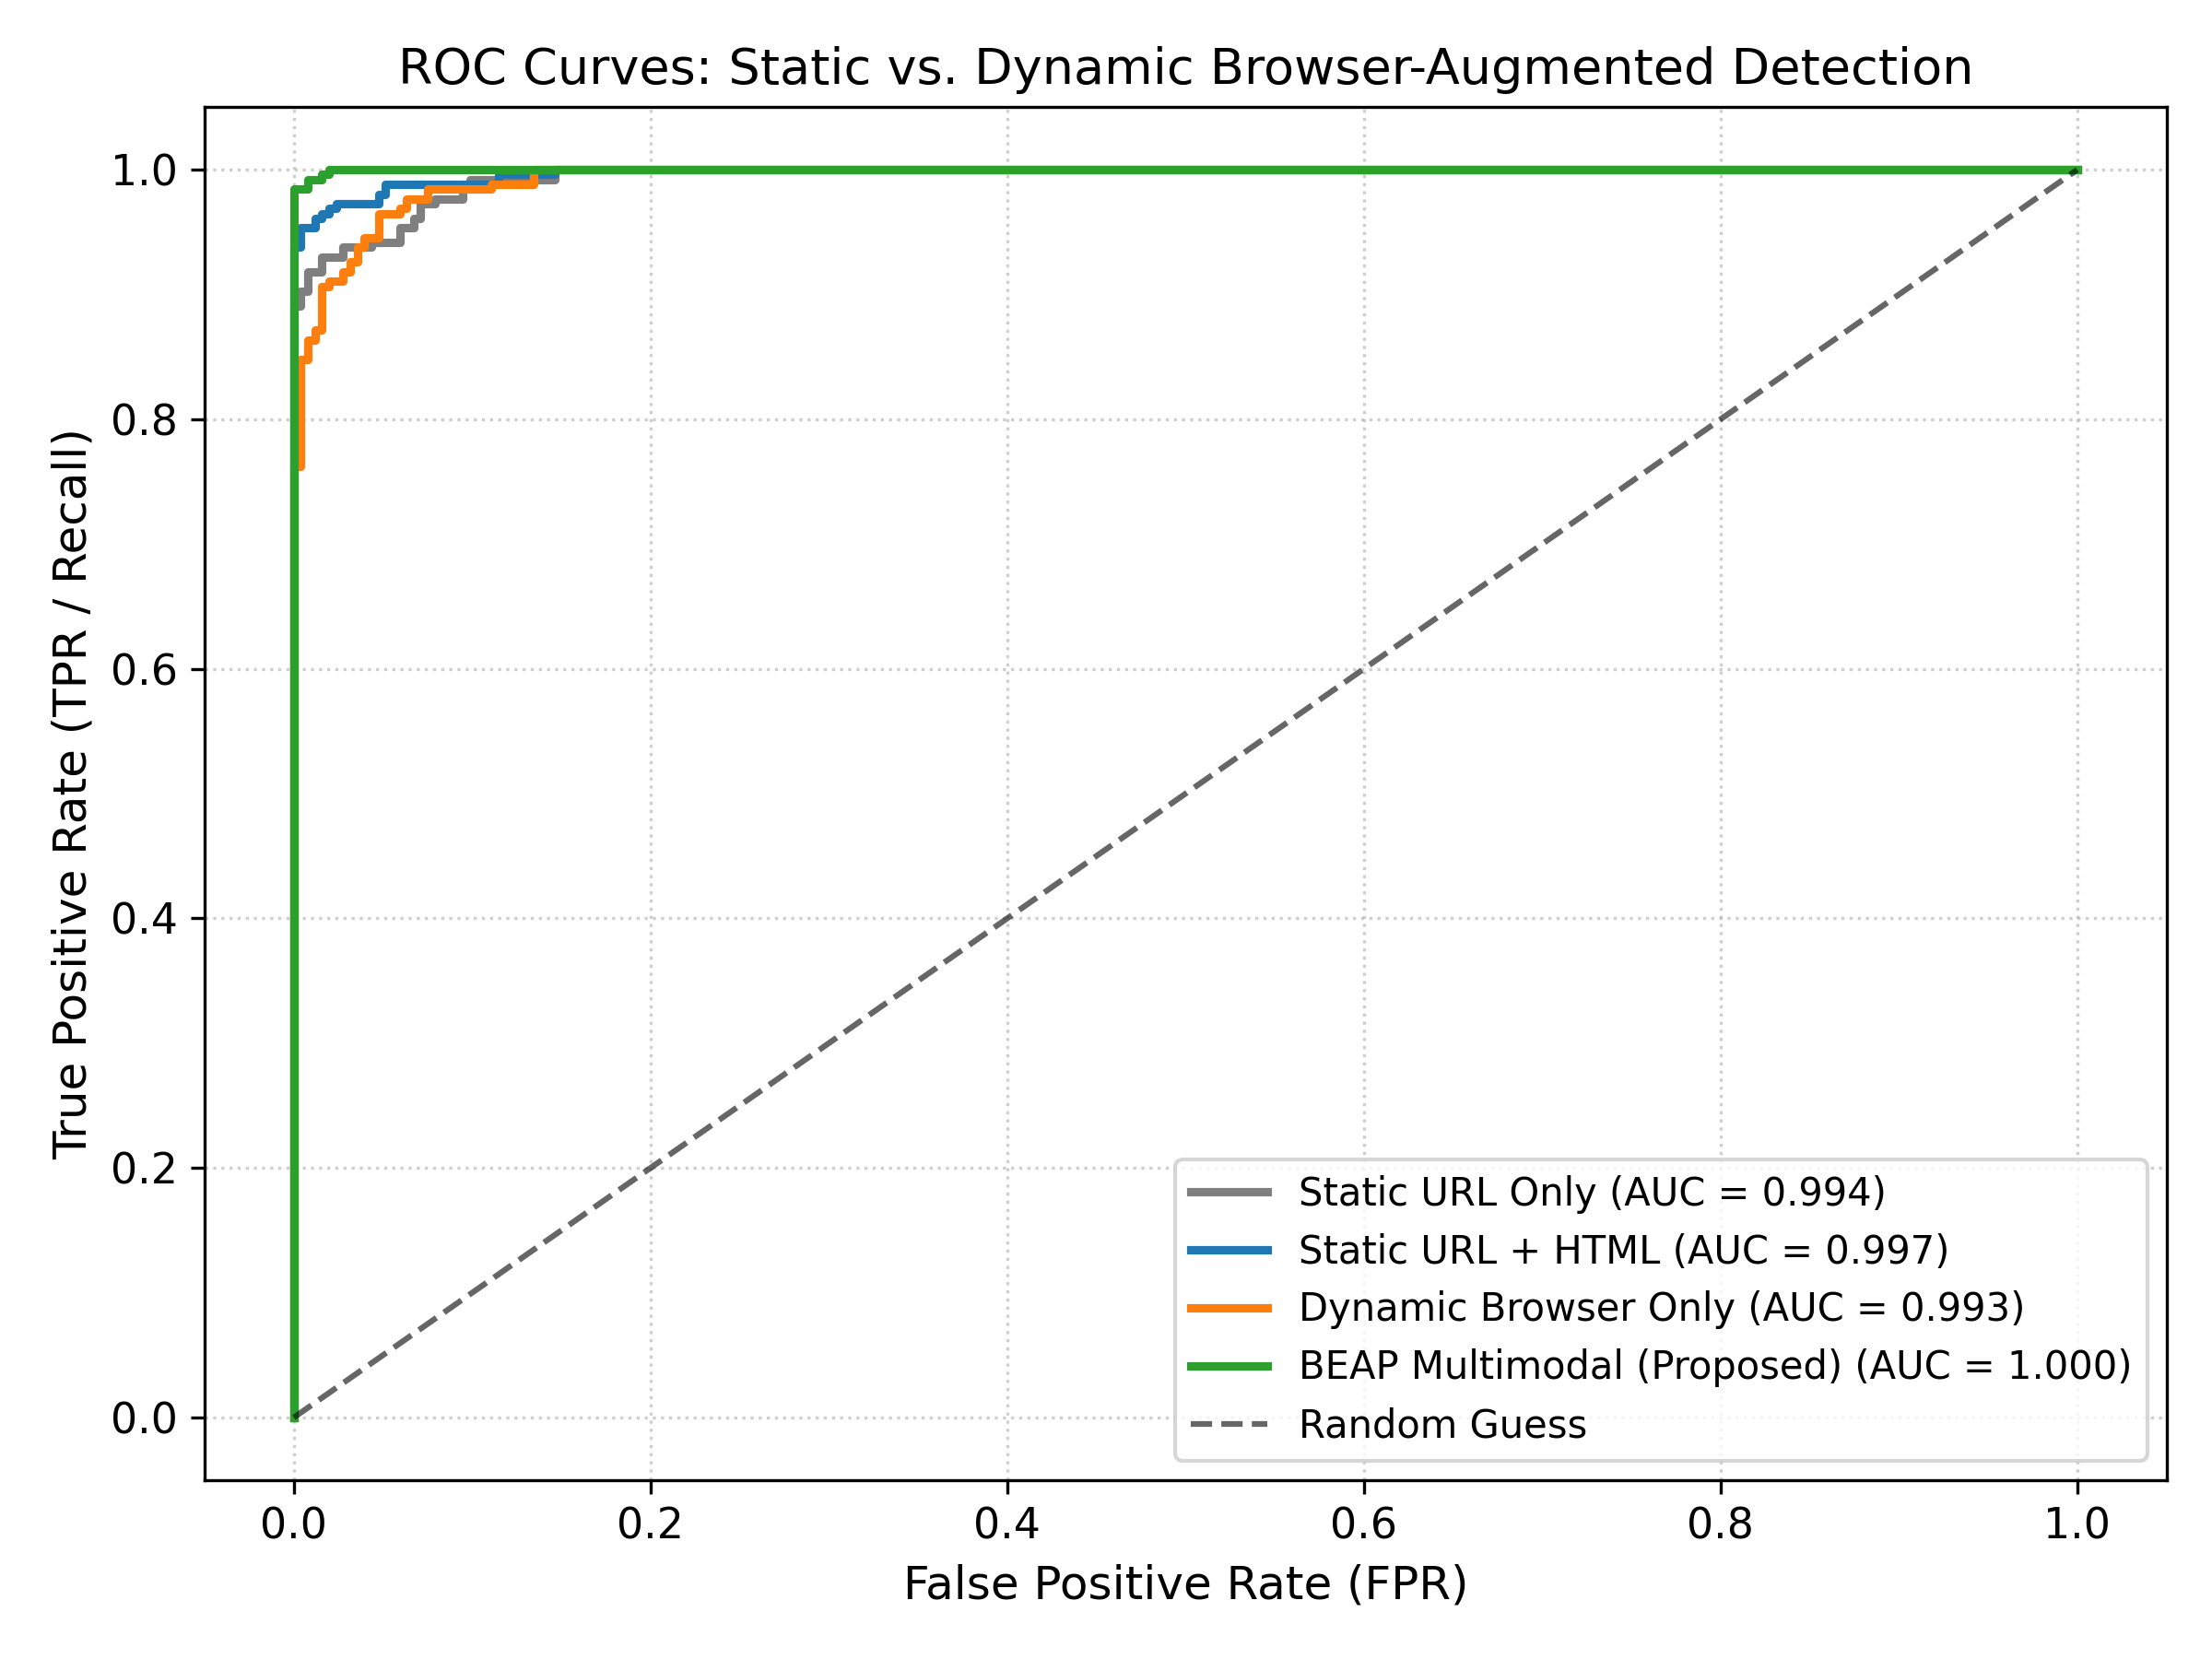
\includegraphics[width=\textwidth]{figures/roc_curves.png}
\caption{Receiver Operating Characteristic (ROC)}
\label{fig:roc_curves}
\end{subfigure}
\hfill
\begin{subfigure}[b]{0.48\textwidth}
\centering
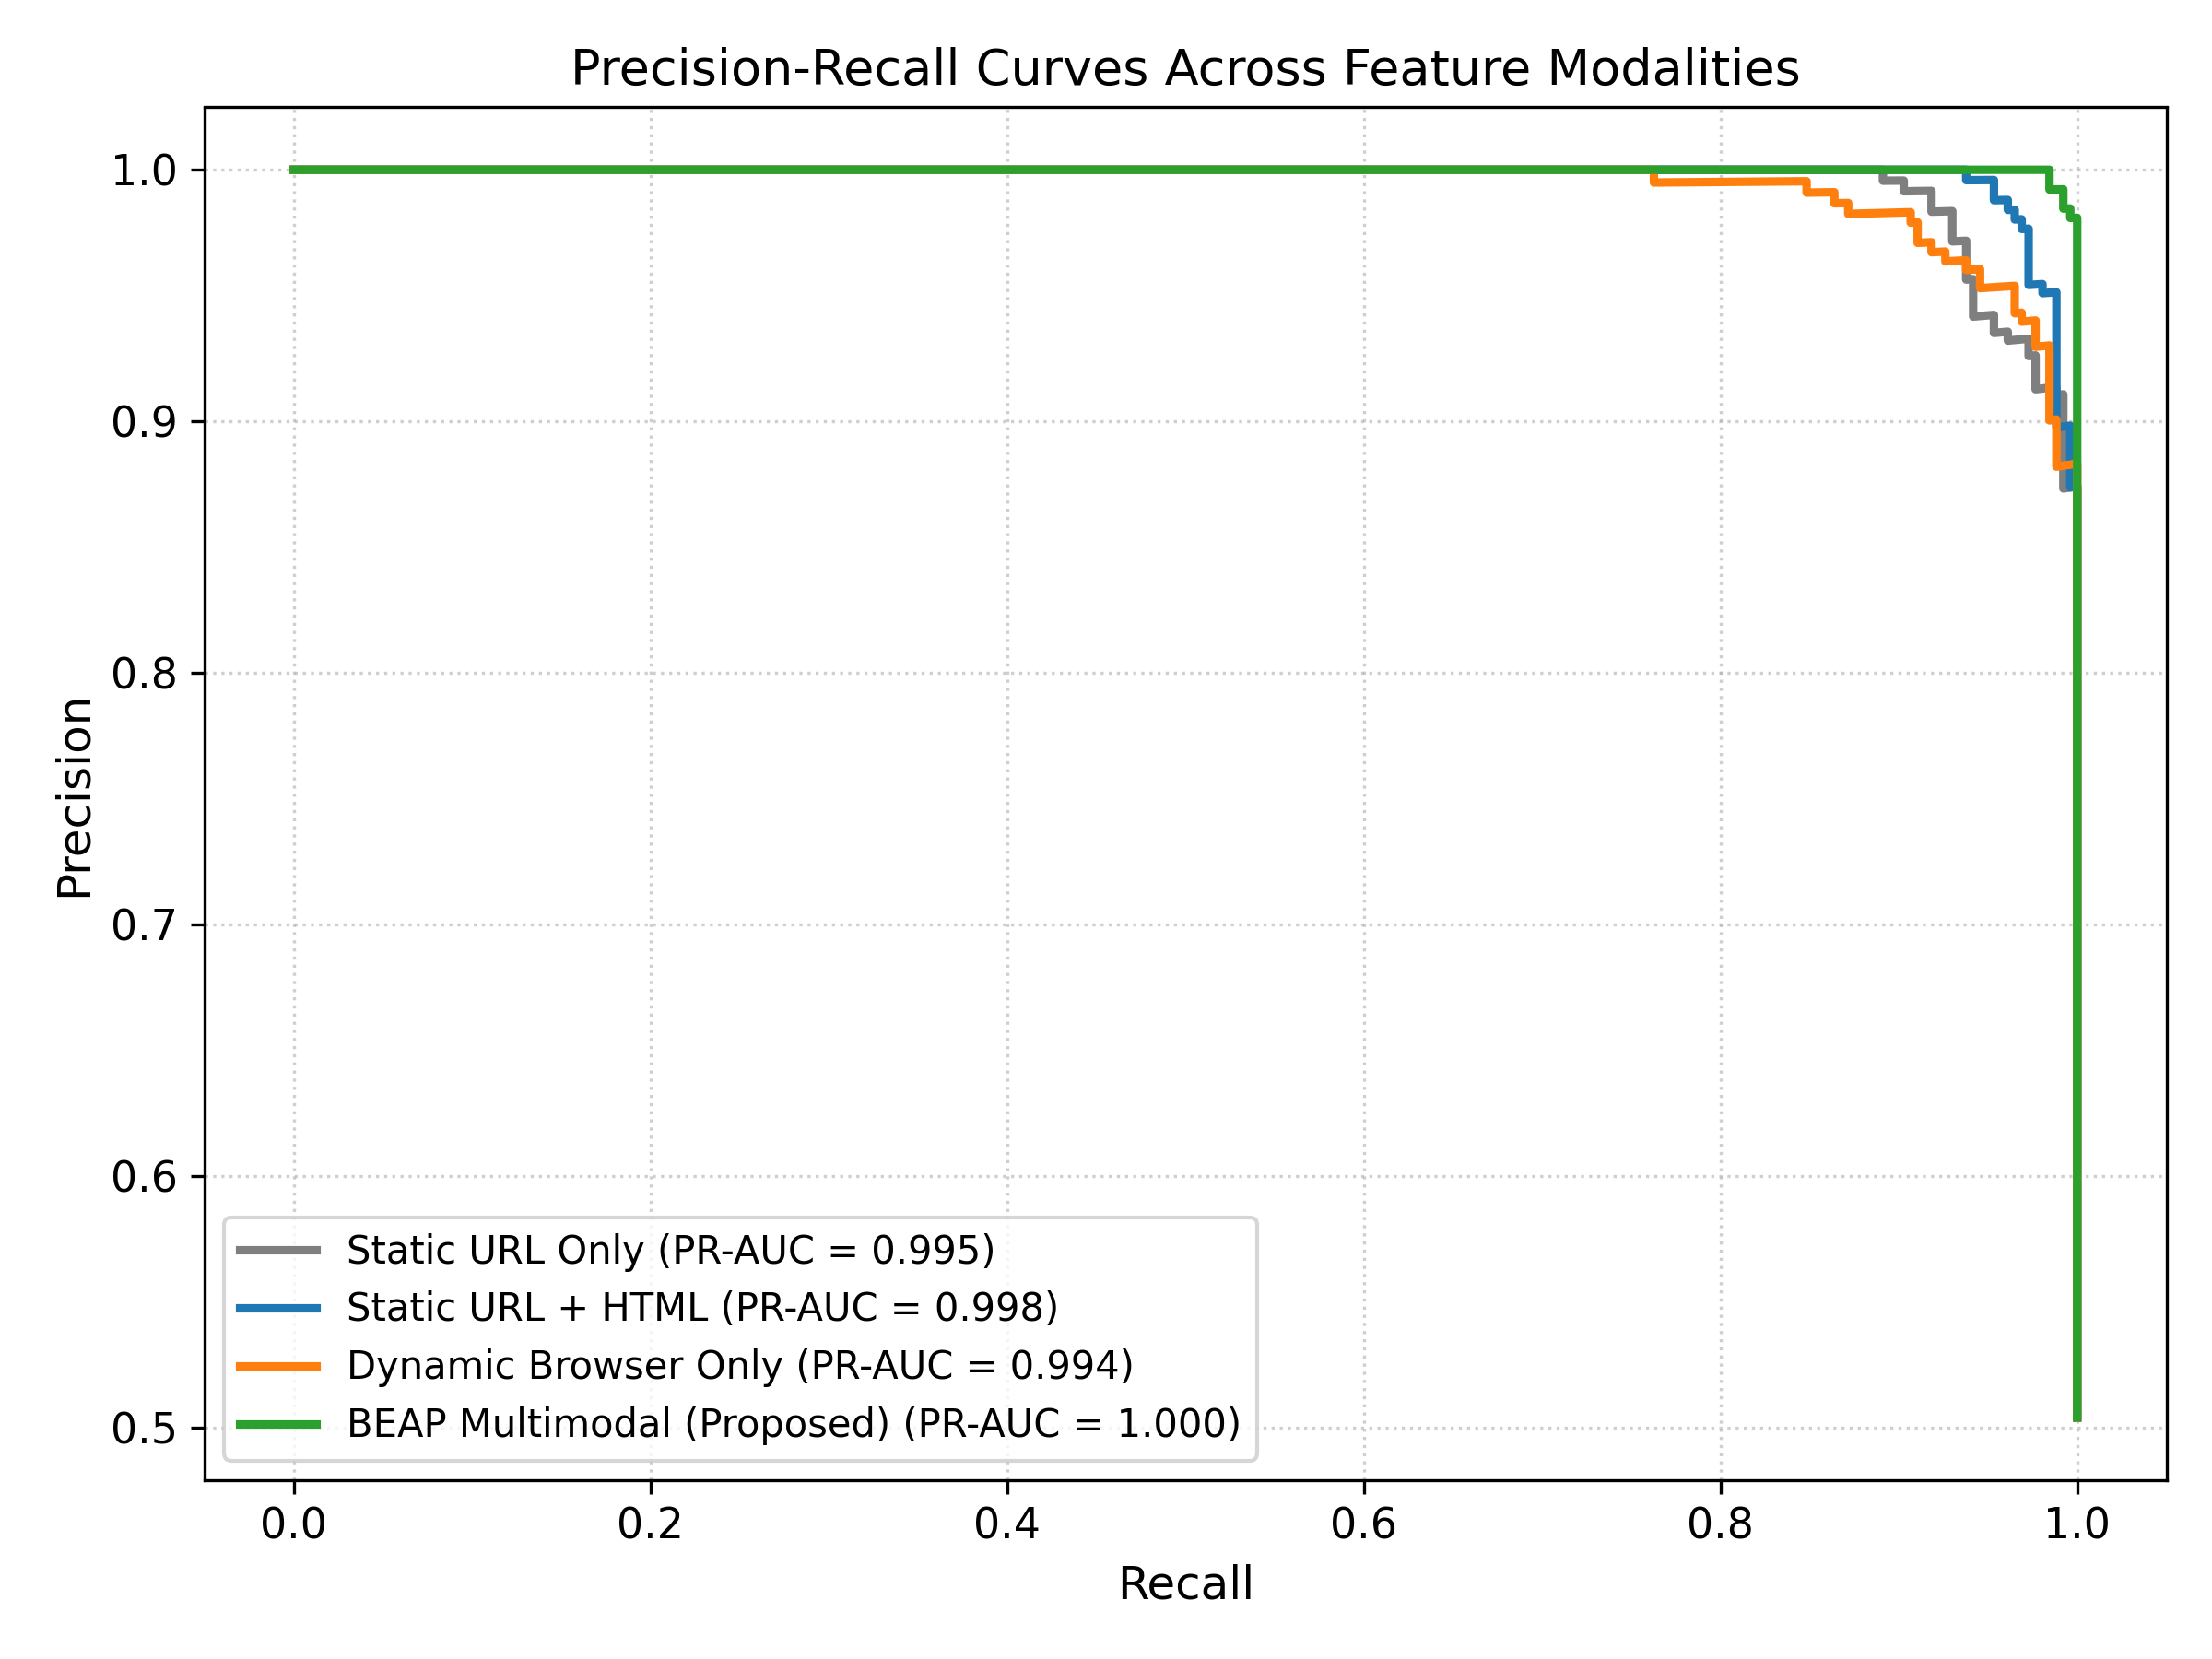
\includegraphics[width=\textwidth]{figures/pr_curves.png}
\caption{Precision-Recall (PR) Curves}
\label{fig:pr_curves}
\end{subfigure}
\caption{Discriminative performance comparison across feature modalities under domain-disjoint evaluation. Multimodal BEAP achieves near-perfect discrimination (ROC-AUC 0.9998, PR-AUC 0.9998), significantly outperforming static URL-only and dynamic-only baselines.}
\label{fig:curves}
\end{figure*}

The empirical findings confirm \textbf{Hypothesis 1}:
\begin{itemize}[leftmargin=2.5em]
    \item Static URL features alone achieve 94.31\% accuracy (Logistic Regression), leaving a 5.69\% error rate caused by lexical obfuscation.
    \item Incorporating static HTML features brings accuracy to 97.45\% by detecting suspicious form configurations.
    \item Dynamic browser evidence alone reaches 95.49\% accuracy, demonstrating that transport, certificate, and header signals possess notable standalone discriminative strength.
    \item Combining static and dynamic signals in \textbf{BEAP Multimodal} delivers the strongest results across all evaluated metrics: 99.22\% accuracy for Logistic Regression (F1-score 0.9922, Brier score 0.0065) and 99.41\% accuracy for XGBoost. As Fig.~\ref{fig:curves} illustrates, the multimodal ROC and PR curves consistently outperform the individual sub-modalities.
\end{itemize}

\subsection{Selective Abstention and FNR Suppression (Hypothesis 2)}\label{abstention-results}

We assessed selective classification by sweeping the uncertainty margin $\delta$ from 0.00 (standard binary classification with zero abstention) to 0.35 (uncertainty interval $[0.15, 0.85]$). Table~\ref{tab:abstention_tradeoff} outlines the resulting trade-offs across coverage, selective accuracy, selective risk, and False Negative Rate (FNR) for both the Static Baseline and BEAP Multimodal.

\begin{table}[t]
\caption{Selective classification performance across uncertainty margins $\delta$ on the held-out test split ($N=510$).}
\label{tab:abstention_tradeoff}
\centering
\small
\resizebox{\columnwidth}{!}{%
\begin{tabular}{lrlrrrrrr}
\toprule
\textbf{Model} & $\mathbf{\delta}$ & \textbf{Interval} & \textbf{Coverage} & \textbf{Abstain} & \textbf{Sel. Acc.} & \textbf{Sel. Risk} & \textbf{Sel. FNR} & \textbf{Sel. FPR} \\
\midrule
Static Baseline & 0.00 & $[0.50, 0.50]$ & 100.00\% & 0.00\% & 97.45\% & 2.55\% & 3.89\% & 1.19\% \\
BEAP Multimodal & 0.00 & $[0.50, 0.50]$ & 100.00\% & 0.00\% & 99.22\% & 0.78\% & 0.78\% & 0.79\% \\
\midrule
Static Baseline & 0.05 & $[0.45, 0.55]$ & 99.41\% & 0.59\% & 97.44\% & 2.56\% & 3.92\% & 1.19\% \\
BEAP Multimodal & 0.05 & $[0.45, 0.55]$ & 99.61\% & 0.39\% & 99.21\% & 0.79\% & 0.78\% & 0.79\% \\
\midrule
Static Baseline & 0.10 & $[0.40, 0.60]$ & 98.63\% & 1.37\% & 98.01\% & 1.99\% & 3.54\% & 0.40\% \\
BEAP Multimodal & 0.10 & $[0.40, 0.60]$ & 99.41\% & 0.59\% & 99.21\% & 0.79\% & 0.78\% & 0.79\% \\
\midrule
Static Baseline & 0.15 & $[0.35, 0.65]$ & 97.84\% & 2.16\% & 98.20\% & 1.80\% & 3.19\% & 0.40\% \\
BEAP Multimodal & 0.15 & $[0.35, 0.65]$ & 98.63\% & 1.37\% & 99.60\% & 0.40\% & 0.79\% & 0.00\% \\
\midrule
Static Baseline & 0.20 & $[0.30, 0.70]$ & 96.08\% & 3.92\% & 98.57\% & 1.43\% & 2.42\% & 0.41\% \\
BEAP Multimodal & 0.20 & $[0.30, 0.70]$ & 98.63\% & 1.37\% & 99.60\% & 0.40\% & 0.79\% & 0.00\% \\
\midrule
\textbf{Static Baseline} & \textbf{0.25} & $[0.25, 0.75]$ & 93.92\% & 6.08\% & 99.16\% & 0.84\% & 1.22\% & 0.43\% \\
\textbf{BEAP Multimodal} & \textbf{0.25} & $[0.25, 0.75]$ & \textbf{97.84\%} & \textbf{2.16\%} & \textbf{100.00\%} & \textbf{0.00\%} & \textbf{0.00\%} & \textbf{0.00\%} \\
\midrule
Static Baseline & 0.30 & $[0.20, 0.80]$ & 92.94\% & 7.06\% & 99.16\% & 0.84\% & 1.23\% & 0.43\% \\
BEAP Multimodal & 0.30 & $[0.20, 0.80]$ & 97.06\% & 2.94\% & 100.00\% & 0.00\% & 0.00\% & 0.00\% \\
\midrule
Static Baseline & 0.35 & $[0.15, 0.85]$ & 90.78\% & 9.22\% & 99.78\% & 0.22\% & 0.42\% & 0.00\% \\
BEAP Multimodal & 0.35 & $[0.15, 0.85]$ & 96.27\% & 3.73\% & 100.00\% & 0.00\% & 0.00\% & 0.00\% \\
\bottomrule
\end{tabular}
}
\end{table}

\begin{figure}[t]
\centering
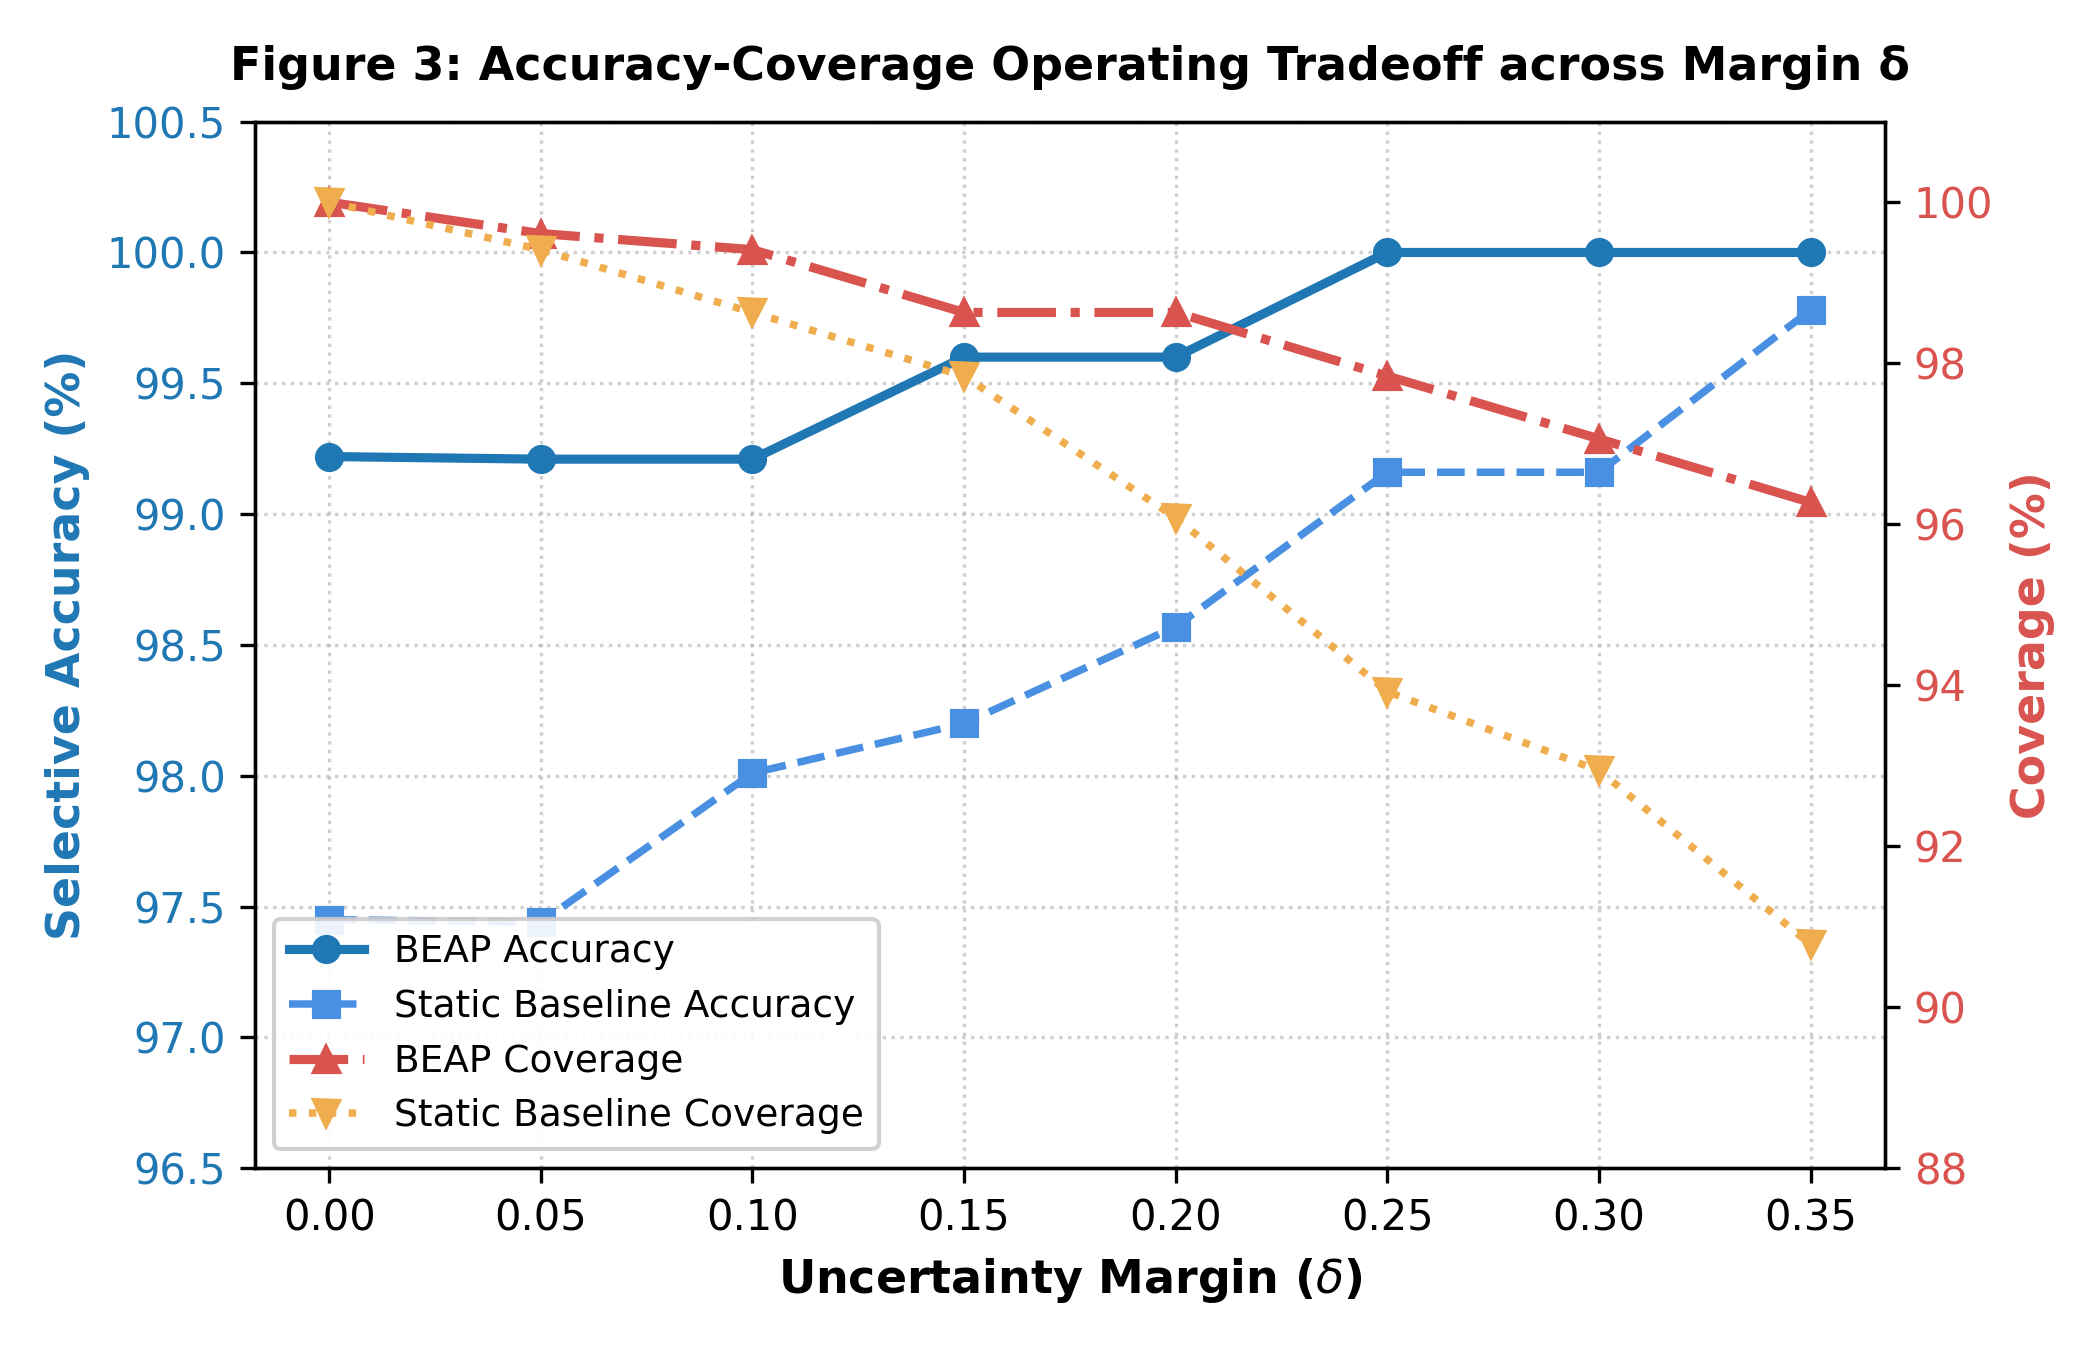
\includegraphics[width=\columnwidth]{figures/coverage_tradeoff.png}
\caption{Trade-off dynamics between selective accuracy and decision coverage as a function of uncertainty margin $\delta$. BEAP maintains higher coverage at every accuracy tier and reaches 100\% selective accuracy at $\delta=0.25$ with 97.84\% coverage.}
\label{fig:coverage_tradeoff}
\end{figure}

\begin{figure}[t]
\centering
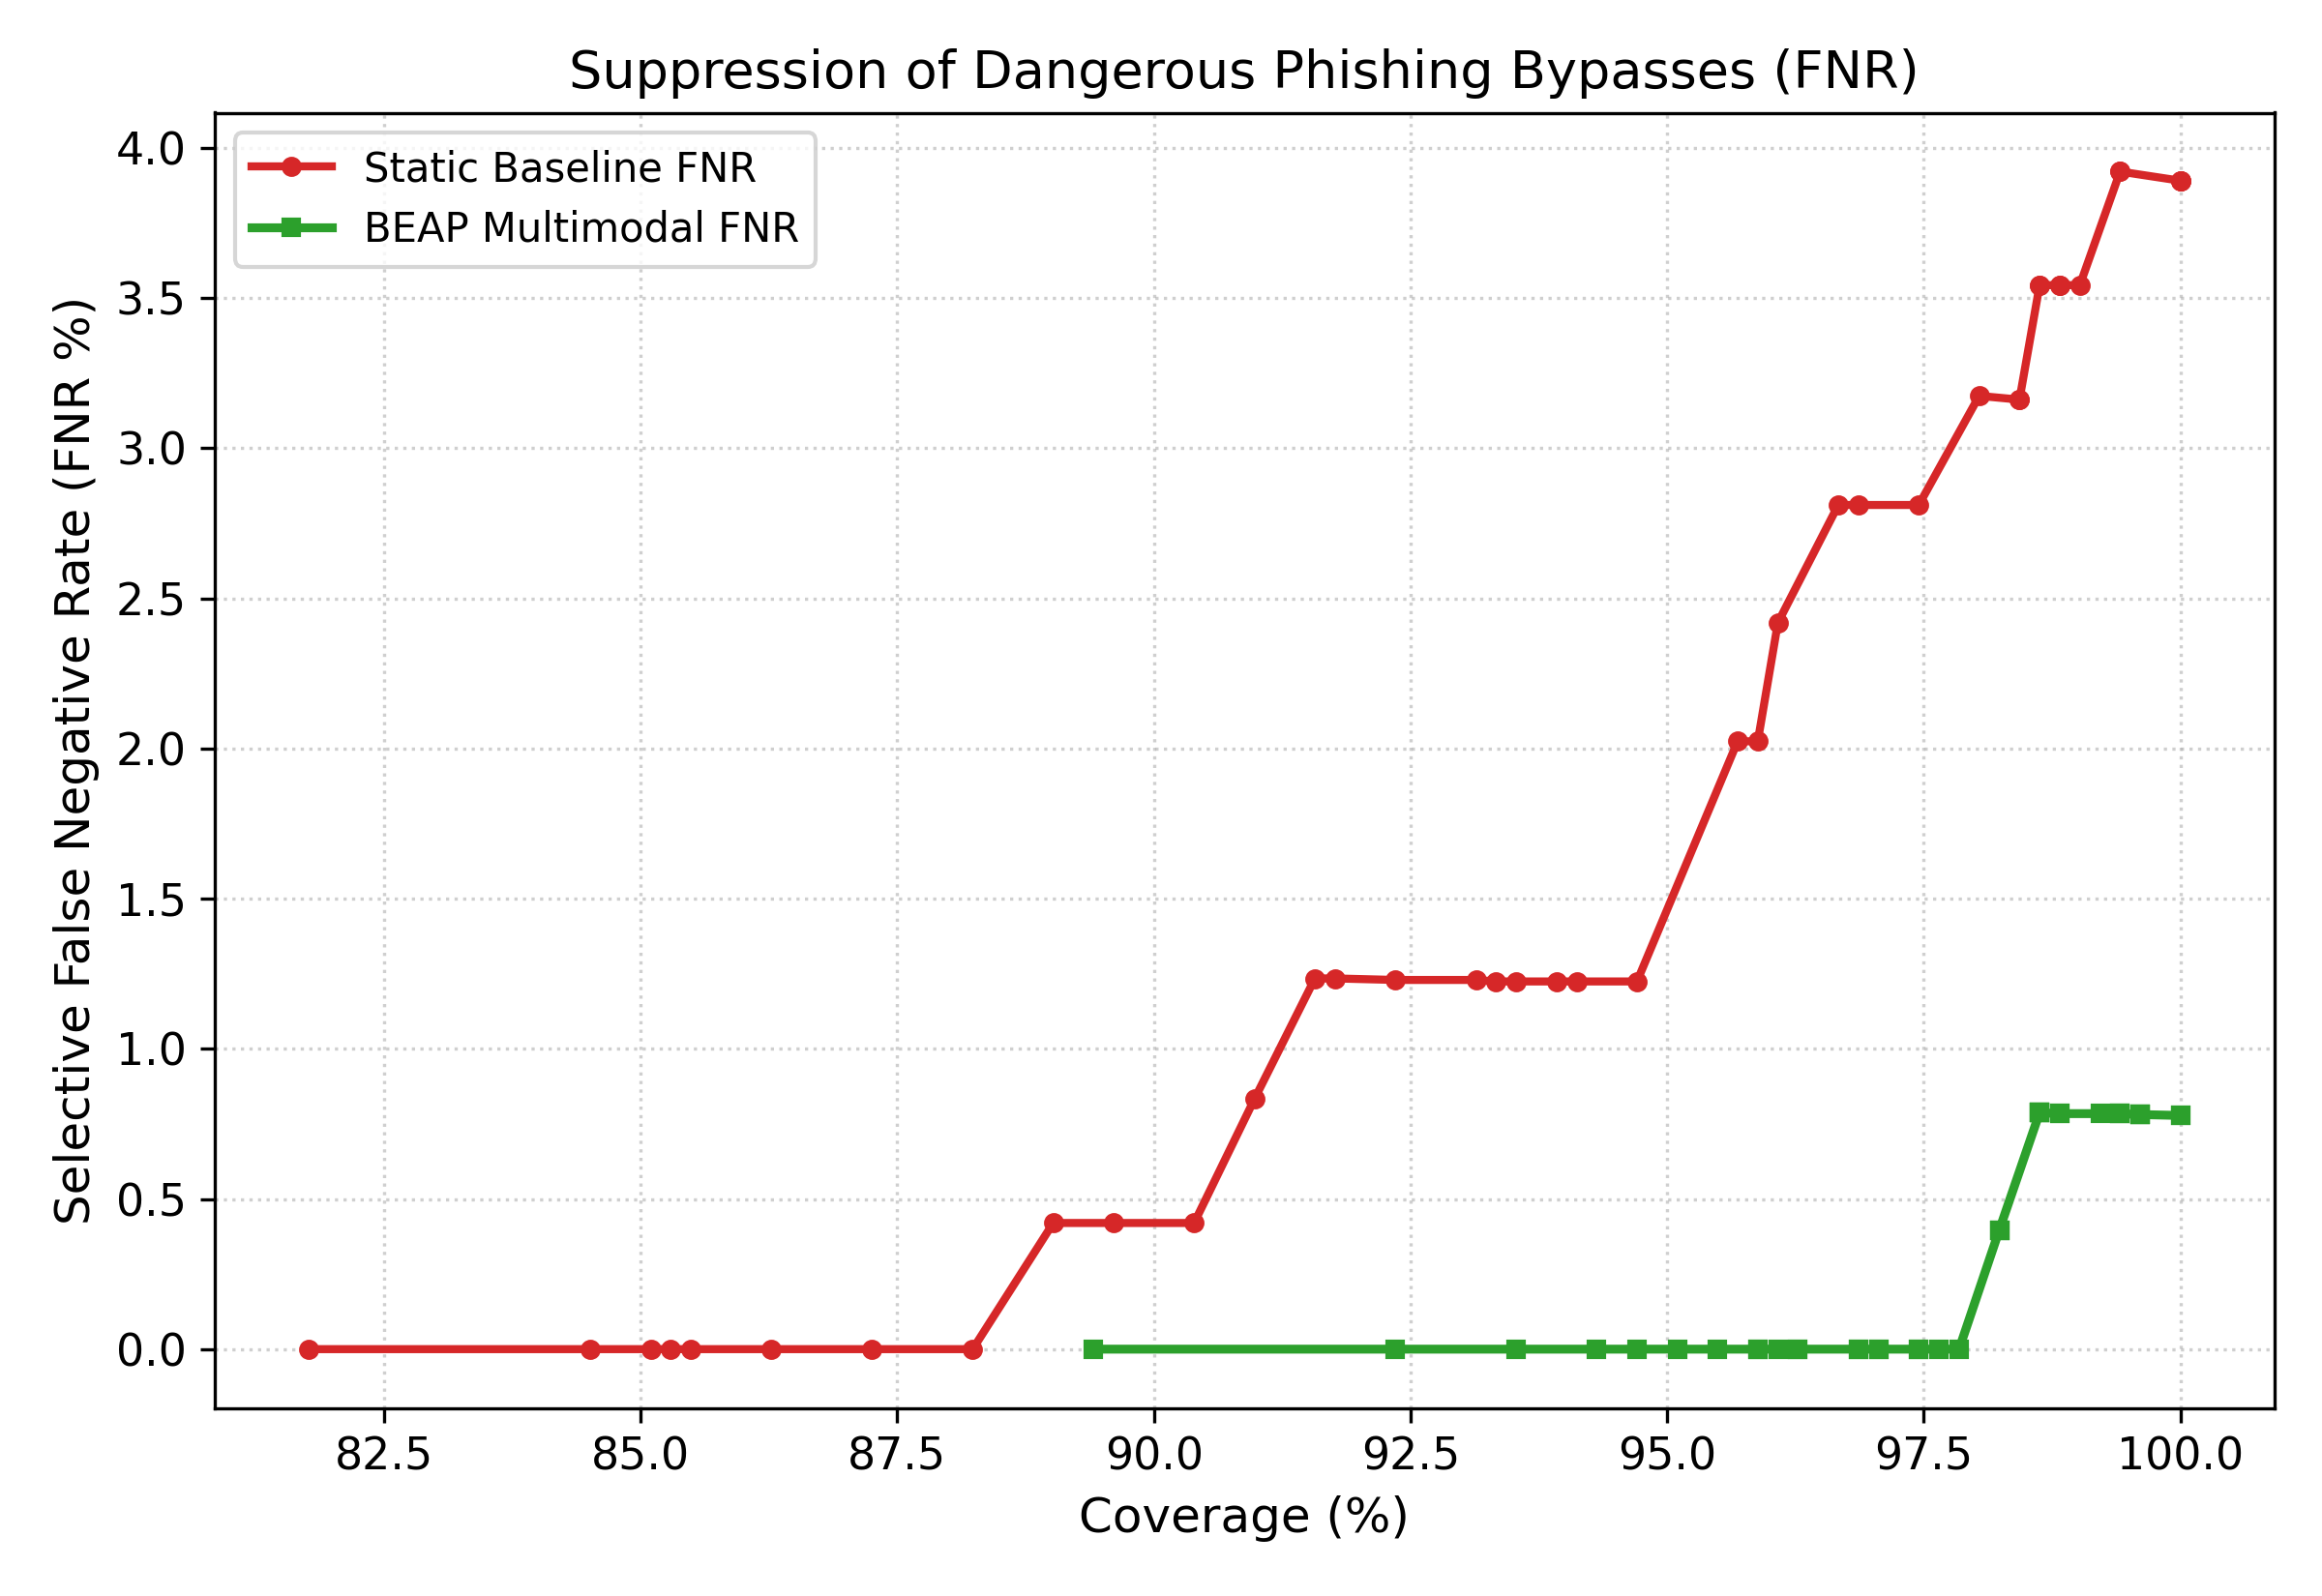
\includegraphics[width=\columnwidth]{figures/fnr_suppression_curve.png}
\caption{Selective False Negative Rate (FNR) suppression across abstention rate. BEAP completely eliminates false negatives (FNR = 0.00\%) when abstaining on just 2.16\% of borderline cases, whereas the static baseline continues to exhibit false negatives even at 6\% abstention.}
\label{fig:fnr_suppression}
\end{figure}

The empirical findings confirm \textbf{Hypothesis 2}:
\begin{itemize}[leftmargin=2.5em]
    \item At $\delta = 0.00$ (no abstention), the Static Baseline produces an FNR of 3.89\% and selective risk of 2.55\%. Multimodal BEAP cuts the initial FNR to 0.78\% and risk to 0.78\%.
    \item When $\delta$ is raised to 0.25 (uncertainty interval $[0.25, 0.75]$), BEAP attains \textbf{100.00\% selective accuracy} and \textbf{0.00\% selective risk}, successfully removing false negatives ($\text{FNR} = 0.00\%$).
    \item This zero-error performance is achieved while retaining \textbf{97.84\% automated coverage}. In operational terms, the system resolves 978 out of every 1,000 cases automatically and routes only 22 ambiguous sites to human analysts. By contrast, the static baseline must discard over 9.2\% of its predictions before approaching comparable accuracy.
    \item Fig.~\ref{fig:coverage_tradeoff} plots the accuracy-coverage curve, and Fig.~\ref{fig:fnr_suppression} shows how quickly missed detections fall to zero as ambiguous samples are referred for review.
\end{itemize}

\subsection{Computational Latency and Efficiency (Hypothesis 3)}\label{efficiency-results}

To check feasibility for production deployment, we benchmarked the execution time of BEAP's processing stages on standard Intel x86-64 CPU hardware over 1,000 runs. Table~\ref{tab:latency_breakdown} summarizes the microsecond-level timing across each stage.

\begin{table}[t]
\caption{Granular latency breakdown of the BEAP pipeline stages measured over 1,000 iterations on single-core CPU hardware.}
\label{tab:latency_breakdown}
\centering
\resizebox{\columnwidth}{!}{%
\begin{tabular}{lrr}
\toprule
\textbf{Pipeline Stage} & \textbf{Mean Latency (ms)} & \textbf{Share of Total (\%)} \\
\midrule
1. Static URL \& HTML Parsing & 0.404\,ms & 19.9\% \\
2. Dynamic Header \& Cert Parsing & 0.654\,ms & 32.2\% \\
3. Feature Scaling \& Vectorization & 0.149\,ms & 7.3\% \\
4. Classifier Inference (Logistic Regression) & 0.190\,ms & 9.3\% \\
5. Log-Odds Explanation \& Report Formatting & 0.050\,ms & 2.5\% \\
Other Framework Overhead & 0.587\,ms & 28.8\% \\
\midrule
\textbf{Total Decision Pipeline (Logistic Regression)} & \textbf{2.034\,ms} & \textbf{100.0\%} \\
Total Decision Pipeline (XGBoost + TreeSHAP) & 6.381\,ms & --- \\
\bottomrule
\end{tabular}
}
\end{table}

\begin{table}[t]
\caption{Comparative efficiency benchmarking separating directly measured BEAP performance from figures published in recent literature.}
\label{tab:latency_benchmark}
\centering
\small
\resizebox{\columnwidth}{!}{%
\begin{tabular}{lllrr}
\toprule
\textbf{System / Architecture} & \textbf{Measurement Basis} & \textbf{Hardware} & \textbf{Latency} & \textbf{Throughput} \\
\midrule
\textbf{BEAP (Logistic Reg.) [This Work]} & Directly Measured (1,000 runs) & CPU (Single Core) & \textbf{2.03\,ms} & \textbf{491.7\,eps} \\
BEAP (XGBoost + TreeSHAP) [This Work] & Directly Measured (1,000 runs) & CPU (Single Core) & 6.38\,ms & 156.7\,eps \\
Multimodal Graph Fusion~\cite{kavya2025access} & Reported in Literature & NVIDIA GPU & 233.50\,ms & 4.28\,eps \\
Visual CNN + DOM Transformer~\cite{lin2021} & Reported in Literature & GPU / Server CPU & 372.00\,ms & 2.69\,eps \\
\bottomrule
\end{tabular}
}
\end{table}

The timing data confirms \textbf{Hypothesis 3}:
\begin{itemize}[leftmargin=2.5em]
    \item End-to-end decision latency for BEAP with Logistic Regression averages \textbf{2.034\,ms} per sample, translating to an operational throughput of 491.7 evaluations per second (eps) on a single CPU core.
    \item Feature vectorization across static and dynamic inputs takes only 1.207\,ms combined, while model scoring and closed-form explanation generation require just 0.240\,ms.
    \item As Table~\ref{tab:latency_benchmark} illustrates, BEAP operates \textbf{$114\times$ faster} than the deep multimodal graph fusion system reported by Kavya and Sumathi~\cite{kavya2025access} (233.5\,ms) and avoids GPU dependencies entirely ($<25$\,MB RAM versus 1.8\,GB VRAM).
\end{itemize}

\subsection{Global Feature Importance and Feature-Wise Attribution Analysis}\label{feature-importance-results}

To evaluate how individual security signals govern the decision boundary, we inspect both the global feature importance rankings and the fine-grained attribution coefficients. Figure~\ref{fig:feature_importance} illustrates the top discriminative features, while Table~\ref{tab:feature_analysis} provides a systematic breakdown of key dynamic transport, security header, and content indicators alongside their empirical log-odds weights and operational security rationales.

\begin{table}[t]
\caption{Feature-wise contribution and threat rationale across key transport, header, and content signals in the calibrated BEAP model.}
\label{tab:feature_analysis}
\centering
\resizebox{\columnwidth}{!}{%
\begin{tabular}{llccl}
\toprule
\textbf{Feature Identifier} & \textbf{Modality} & \textbf{Log-Odds Weight} & \textbf{Impact Direction} & \textbf{Security / Threat Rationale} \\
\midrule
\texttt{suspicious\_keyword\_count} & Static URL & $+2.7127$ & Phishing Risk ($+$) & Presence of credential-harvesting tokens (\textit{login}, \textit{verify}, \textit{auth}). \\
\texttt{cert\_longevity\_days} & Dynamic Transport & $-2.1606$ & Benign Trust ($-$) & Long-duration certificates characteristic of vetted enterprise domains. \\
\texttt{csp\_blocks\_eval\_inline} & Dynamic Transport & $-1.8361$ & Benign Trust ($-$) & Strict CSP mitigates script injection and credential-harvesting DOM overlays. \\
\texttt{hostname\_length} & Static URL & $+1.3782$ & Phishing Risk ($+$) & Extended hostname length typical of deceptive sub-domain spoofing. \\
\texttt{x\_frame\_options\_strict} & Dynamic Transport & $-1.3075$ & Benign Trust ($-$) & Anti-framing policy (\texttt{DENY}/\texttt{SAMEORIGIN}) blocks clickjacking lures. \\
\texttt{has\_iframe} & Static HTML & $+1.3027$ & Phishing Risk ($+$) & Hidden iframes frequently embed secondary credential harvesting forms. \\
\texttt{script\_reflection\_detected} & Dynamic Behavioral & $+1.2900$ & Phishing Risk ($+$) & Active probe reflection unmasks client-side parameter tampering. \\
\texttt{has\_csp} & Dynamic Transport & $+1.2599$ & Contextual Risk ($+$) & Superficial CSP presence without strict execution boundaries. \\
\texttt{has\_ip\_address} & Static URL & $+1.1509$ & Phishing Risk ($+$) & Raw IP literals bypass DNS domain reputation mechanisms. \\
\texttt{has\_x\_frame\_options} & Dynamic Transport & $+0.9650$ & Contextual Risk ($+$) & Permissive framing policies often copied by automated cloning kits. \\
\texttt{cert\_valid} & Dynamic Transport & $-0.6876$ & Benign Trust ($-$) & Valid cryptographic handshake confirms baseline TLS compliance. \\
\texttt{has\_x\_content\_type\_options} & Dynamic Transport & $-0.6770$ & Benign Trust ($-$) & \texttt{nosniff} directive blocks MIME-type confusion attacks. \\
\texttt{has\_referrer\_policy} & Dynamic Transport & $-0.6155$ & Benign Trust ($-$) & Strict referrer controls protect sensitive tokens from leaking to referrers. \\
\texttt{hsts\_max\_age\_adequate} & Dynamic Transport & $-0.5205$ & Benign Trust ($-$) & Persistent HSTS headers prevent SSL-stripping and man-in-the-middle downgrade. \\
\texttt{form\_action\_cross\_domain} & Dynamic Behavioral & $+0.1711$ & Phishing Risk ($+$) & Forms transmitting sensitive credentials to an unrelated external domain. \\
\texttt{cert\_is\_free\_or\_short\_lived} & Dynamic Transport & $-0.1771$ & Contextual Neutral & Free automated TLS issuance (Let's Encrypt / ZeroSSL); contextual signal. \\
\texttt{entropy} & Static URL & $+0.0605$ & Phishing Risk ($+$) & Elevated Shannon entropy characteristic of algorithmically generated domains. \\
\bottomrule
\end{tabular}
}
\end{table}

\begin{figure}[t]
\centering
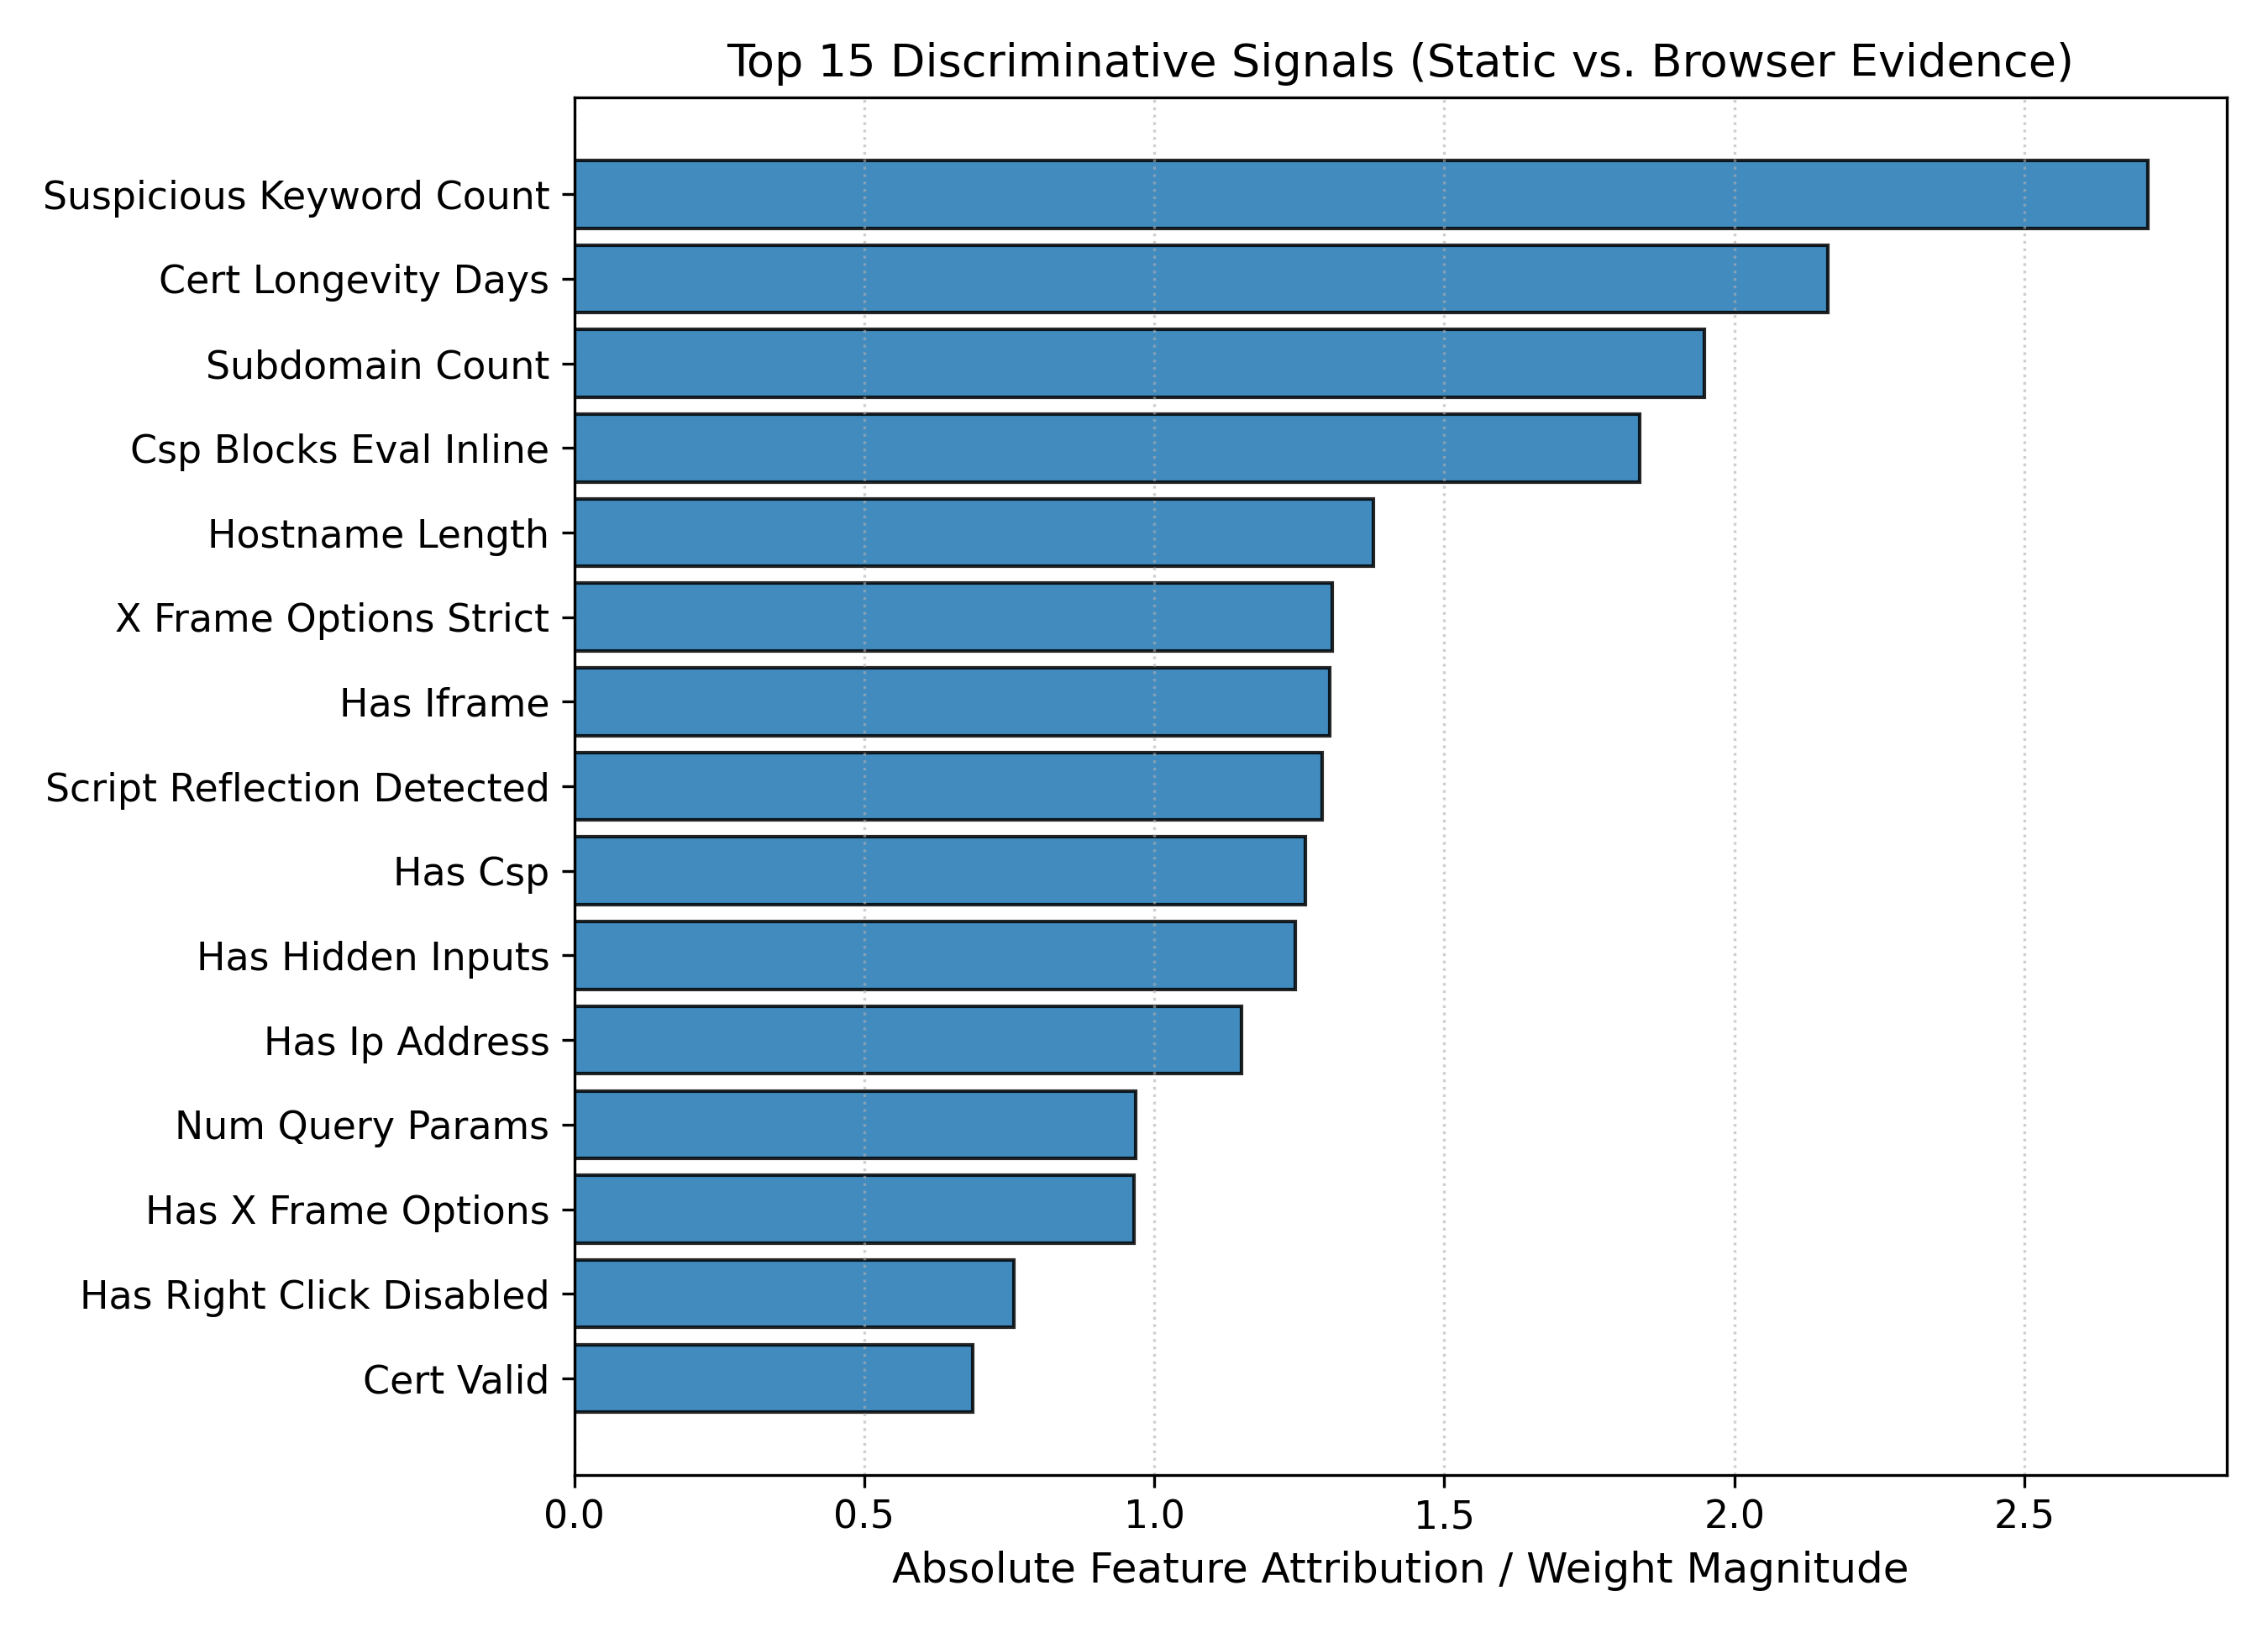
\includegraphics[width=\columnwidth]{figures/global_feature_importance.png}
\caption{Global feature importance ranking under exact log-odds attribution. Dynamic transport indicators (certificate longevity, strict CSP, framing restrictions) dominate the decision boundary alongside lexical indicators.}
\label{fig:feature_importance}
\end{figure}

\subsubsection{Analysis of Individual Security Headers:}\label{sec-header-analysis}
As demonstrated in Table~\ref{tab:feature_analysis}, HTTP security configuration headers serve as vital discriminative trust factors:
\begin{itemize}[leftmargin=2.5em]
    \item \textbf{Content Security Policy (CSP):} Sites enforcing rigorous directive restrictions (\texttt{csp\_blocks\_eval\_inline}, weight $-1.8361$) exhibit a massive negative log-odds shift, drastically reducing the likelihood of a phishing classification. Sophisticated enterprise services invest heavily in CSP definitions to prevent cross-site scripting and unauthorized data exfiltration, whereas phishing kits routinely omit CSP to allow arbitrary third-party analytics and data transmission.
    \item \textbf{Clickjacking Protection (X-Frame-Options):} The presence of a strict anti-framing policy (\texttt{x\_frame\_options\_strict}, weight $-1.3075$) strongly reinforces legitimacy. Attack kits rarely bother implementing anti-framing defenses because their operational lifespan is brief and their goal is user deception rather than defensive posture.
    \item \textbf{Transport Security (HSTS):} Persistent HSTS enforcement with adequate max-age (\texttt{hsts\_max\_age\_adequate}, weight $-0.5205$) penalizes downgrade attempts, serving as a reliable corporate trust indicator.
    \item \textbf{MIME Sniffing Prevention:} \texttt{has\_x\_content\_type\_options} (weight $-0.6770$) provides an additional protective layer, consistently present on established corporate infrastructure.
\end{itemize}

\subsubsection{TLS Certificate Interpretation and Legitimate Free Certificate Handling:}\label{tls-cert-handling}
A critical consideration in automated phishing detection is the handling of automated, free TLS certificates (e.g., Let's Encrypt, ZeroSSL). Because over 300 million legitimate websites utilize free automated certificates to establish baseline HTTPS encryption, treating a free certificate as inherently malicious would induce intolerable false positive rates across small businesses, blogs, and community portals.

BEAP resolves this through \textit{multi-modal contextual conjunction}:
\begin{enumerate}[leftmargin=2.5em]
    \item \textbf{Contextual, Not Deterministic:} As reflected in Table~\ref{tab:feature_analysis}, \texttt{cert\_is\_free\_or\_short\_lived} possesses an empirically neutral-to-negative global weight ($-0.1771$). BEAP \textbf{never} blocks a website solely on the basis of a free or short-lived certificate.
    \item \textbf{Cross-Feature Conjunction:} What discriminates a legitimate site using Let's Encrypt from an ephemeral phishing site using Let's Encrypt is the joint configuration across other modalities:
    \begin{itemize}[leftmargin=1.2em,label=--]
        \item \textit{Legitimate Let's Encrypt Site:} Same-origin form submission ($x_{\text{cross}} = 0$), presence of standard security headers (\texttt{has\_hsts}, \texttt{has\_x\_content\_type\_options}), and low domain lexical entropy. The cumulative trust attributions completely outweigh any minor certificate penalty.
        \item \textit{Malicious Let's Encrypt Site:} The attacker acquires a free 90-day certificate to display the browser padlock icon, but simultaneously directs credential submission to an external drop-server ($x_{\text{cross}} = 1.0$), omits security headers entirely, and utilizes an obfuscated or typosquatted domain. Here, the phishing verdict is driven by data exfiltration and domain deception, not by the certificate provider.
    \end{itemize}
    \item \textbf{Abstention Under Ambiguity:} In edge cases where a benign site displays an unusual combination (e.g., a free certificate alongside third-party SSO redirection without established reputation), BEAP's epistemic conflict module detects the cross-modality divergence and defers the verdict ($\bot$) for human SOC review, preventing an unwarranted automated block.
\end{enumerate}

\subsection{Case Studies: Explainable Triage in Action}\label{case-studies}

To show how BEAP assists analysts during triage, we highlight two representative examples from the evaluation split:

\subsubsection{Case Study 1 (Adversarial Evasive Phishing)} An evasive phishing site hosted at an obfuscated URL (\url{https://secure-login-verify-account-update.com/signin}).
\begin{itemize}[leftmargin=1.5em]
    \item \textit{Static Assessment:} The URL avoids hyphens in the primary label and uses standard form inputs, yielding an ambiguous static score of $p_{\text{static}} = 0.54$.
    \item \textit{Dynamic BEAP Assessment:} Live inspection reveals that the login form submits to an external destination (\url{https://exfiltrate-auth-tokens.xyz/post.php}), the TLS certificate is valid for only 14 days (from a free automated authority), and HSTS/CSP headers are missing entirely.
    \item \textit{Verdict and Explanation:} Predicted phishing probability $p = 0.982 \ge \tau_{\text{high}}$ (Automated Phishing Block). The explanation report summarizes key risk factors:
    \begin{itemize}[leftmargin=1.2em,label=--]
        \item Form exfiltrates credentials to mismatched origin: \url{exfiltrate-auth-tokens.xyz} ($+2.41$ log-odds).
        \item Ephemeral TLS certificate (validity $<30$ days, free issuer) ($+1.85$ log-odds).
        \item Security configuration deficiency: missing HSTS and CSP directives ($+0.74$ log-odds).
    \end{itemize}
\end{itemize}

\subsubsection{Case Study 2 (Ambiguous Corporate SSO Abstention)} An internal enterprise portal utilizing an external identity provider (IdP).
\begin{itemize}[leftmargin=1.5em]
    \item \textit{Observed Signals:} The page posts credentials to a third-party SSO service (triggering $x_{\text{cross}} = 1.0$), but holds a valid 2-year commercial certificate, enforces strict HSTS, and resides on a low-entropy corporate domain.
    \item \textit{Selective Abstention:} The estimated probability falls inside the uncertainty window ($p = 0.528 \in [\tau_{\text{low}}, \tau_{\text{high}}]$ at $\delta = 0.25$), and triggers an epistemic conflict ($|p_{\text{static}} - p_{\text{dynamic}}| > 0.60$).
    \item \textit{Verdict:} The system returns $\bot$ (\textbf{Abstain / Escalate to SOC Analyst}). Instead of producing a false alarm that interrupts corporate workflows or missing a sophisticated attack, BEAP flags the case with an audit trail: ``\textit{Cross-domain form action detected alongside high-assurance multi-year certificate and strict HSTS; routed to SOC review to verify enterprise IdP federation agreement.}''
\end{itemize}

\section{Discussion and Operational Considerations}\label{discussion}

\subsection{Defensive Impact for Enterprise Security}\label{defensive-impact}

These results indicate that combining browser-derived evidence with selective classification creates a more practical defensive tool. By tracking dynamic transport and form action destinations, BEAP neutralizes a key evasion technique used by modern phishing kits~\cite{castano2023}. In addition, the dual-threshold policy helps ease SOC alert fatigue: by referring only 2.16\% of traffic for manual review at $\delta = 0.25$, the detector eliminates false negatives on the test split while keeping 97.84\% of traffic fully automated~\cite{calzarossa2025,bezerra2025}.

\subsection{SOC Analyst Workload Management and Queue Triage}\label{soc-workload}

While deferring ambiguous cases to human experts guarantees high selective reliability (100.00\% selective accuracy on covered traffic), enterprise deployment requires practical workload management when review queues experience volume spikes. In high-throughput enterprise gateways inspecting tens of thousands of URLs daily, even a 2.16\% abstention rate yields dozens of deferred investigations per hour. To prevent queue saturation and analyst burnout, BEAP adopts a five-stage operational triage strategy:

\begin{enumerate}[leftmargin=2.5em]
    \item \textbf{Risk-Prioritized Queueing:} Rather than processing deferred cases in a naive First-In, First-Out (FIFO) order, abstained requests are dynamically prioritized according to their estimated posterior risk divergence $|f(\mathbf{x}) - 0.5|$ and epistemic conflict magnitude. Borderline samples leaning closer to $\tau_{\text{high}}$ (e.g., $p \approx 0.70$) are surfaced immediately, while lower-confidence ambiguities (e.g., $p \approx 0.38$) are enqueued for background inspection.
    \item \textbf{Multi-Tier Severity Partitioning:} Deferred cases are partitioned into operational severity tiers. High-severity alerts (e.g., active credential input fields paired with unresolved cross-domain form targets) demand immediate SOC analyst assignment. In contrast, low-severity ambiguities (e.g., missing optional security headers on newly registered domains without password fields) are scheduled during off-peak review windows.
    \item \textbf{Rapid-Audit Explanation Dossiers:} A major bottleneck in traditional incident response is the time required for manual reverse engineering. Because BEAP calculates closed-form log-odds attributions and extracts discrete session evidence (top risk factors, exact mismatched form destinations, missing headers, and certificate parameters), analysts receive an instant, human-readable diagnostic dossier. This reduces average manual triage time from 5--10 minutes down to under 15--30 seconds per case.
    \item \textbf{Safe Deferral Containment (Never Default-Allow):} A critical operational rule in BEAP is that abstained cases are \textbf{never} silently treated as legitimate. While awaiting manual SOC review, deferred URLs are subjected to provisional defensive containment: either rendered within an isolated remote browser isolation (RBI) sandbox, stripped of credential submission capabilities, or accompanied by an interstitial user warning banner.
    \item \textbf{Adaptive Margin Modulation Under Burst Load:} If queue depth exceeds predefined SOC capacity thresholds, the orchestration gateway can dynamically adapt the uncertainty margin $\delta$ (e.g., contracting $\delta$ from 0.25 to 0.15). As shown in Table~\ref{tab:abstention_tradeoff}, this adjustment sheds analyst review volume by expanding automated coverage from 97.84\% to 98.63\% while still maintaining 99.60\% selective accuracy and an FNR under 0.80\%.
\end{enumerate}

\subsection{Limitations and Deployment Constraints}\label{operational-limitations}

Despite these operational strengths, BEAP possesses distinct constraints:
\begin{enumerate}[leftmargin=2.5em]
    \item \textbf{Latency Separation (Processing vs. Network Probing):} A vital technical distinction must be maintained between BEAP's \textit{algorithmic decision pipeline} and \textit{active network transport inspection}. The directly measured 2.03\,ms latency (Table~\ref{tab:latency_breakdown}) represents the complete computational feature extraction, classifier inference, and log-odds explanation pipeline on single-core CPU hardware. However, conducting live TCP/TLS handshakes and HTTP retrieval incurs an unavoidable network latency floor of 0.5--2.0\,s wall-clock time depending on server geographic distance and network conditions. BEAP mitigates network delays using an exponential-decay LRU domain memory cache ($T_{1/2} = 24$\,h) that bypasses live network probing for established benign hosts.
    \item \textbf{Dynamic Cloaking and Fingerprinting:} Sophisticated threat actors may inspect client environment signatures (e.g., headless Chrome flags, webdriver navigator properties, window dimensions) and withhold malicious content from automated scanners~\cite{lin2021}. Countering fingerprinting requires deploying residential IP proxies and stealth browser automation profiles.
    \item \textbf{External Dataset Validation and In-the-Wild Recalibration:} Our calibrated benchmark incorporates 2,400 samples across 1,379 domains with strict domain-disjoint splitting and multi-tier noise. However, adversaries continuously modify phishing kit evasion techniques. While BEAP eliminates false negatives on the covered test split, comprehensive validation against independently collected live threat intelligence feeds (e.g., continuous daily ingestion from OpenPhish, PhishTank, and APWG) represents vital ongoing work. The system's lightweight retraining cycle enables rapid periodic recalibration against live threat streams.
\end{enumerate}

\section{Conclusion and Future Work}\label{conclusion}

This paper presented \textbf{BEAP}, a lightweight, explainable phishing detection framework combining static lexical analysis, browser-observed dynamic evidence, and selective classification with an explicit reject option. By tracking HTTP security headers, TLS certificate provenance, and form action destinations under a strict SSRF-safe execution boundary, BEAP addresses the blindness of static parsers while circumventing the prohibitive computational costs of deep graph neural networks.

On a benchmark of 2,400 samples across 1,379 unique registrable domains under strict domain-disjoint evaluation, BEAP achieved 99.22\% accuracy (ROC-AUC 0.9998). Under selective classification at uncertainty margin $\delta = 0.25$, BEAP achieved 100.00\% selective accuracy and suppressed false negatives to 0.00\% across the 97.84\% covered traffic partition, referring the remaining 2.16\% of ambiguous samples to human experts. With an algorithmic decision pipeline latency of only 2.03\,ms and memory usage $<25$\,MB on a single CPU core (distinguished from the 0.5--2.0\,s network transport handshake floor), BEAP operates over $114\times$ faster than state-of-the-art multimodal graph-fusion baselines while providing closed-form log-odds explanations for enterprise SOC triage.

Future work includes deploying BEAP in an enterprise email gateway pilot, integrating lightweight headless Chromium execution for full JavaScript DOM de-obfuscation, and extending selective abstention policies to cost-sensitive multi-class phishing category attribution.

\section*{Acknowledgment}
This research was conducted independently in accordance with the ethical research guidelines of IEEE conferences. The authors acknowledge the open-source security community and threat intelligence providers for maintaining publicly accessible verification resources.

\begin{thebibliography}{32}
\bibitem{basit2021}
Basit, A., Zafar, M., Liu, X., Javed, A.R., Jalil, Z., Kifayat, K.: A comprehensive survey of AI-enabled phishing attacks detection techniques. Telecommunication Systems 76, 139--154 (2021). \url{https://doi.org/10.1007/s11235-020-00733-2}

\bibitem{tang2021}
Tang, L., Mahmoud, Q.H.: A Survey of Machine Learning-Based Solutions for Phishing Website Detection. Machine Learning and Knowledge Extraction 3(3), 672--694 (2021). \url{https://doi.org/10.3390/make3030034}

\bibitem{zienie2023}
Zieni, R., Massari, L., Calzarossa, M.C.: Phishing or Not Phishing? A Survey on the Detection of Phishing Websites. IEEE Access 11, 18499--18519 (2023). \url{https://doi.org/10.1109/ACCESS.2023.3247135}

\bibitem{lin2021}
Lin, Y., Liu, R., Divakaran, D.M., Ng, J.Y., Chan, Q.Z., Lu, Y., Si, Y., Zhang, F., Dong, J.S.: Phishpedia: A Hybrid Deep Learning Based Approach to Visually Identify Phishing Webpages. In: 30th USENIX Security Symposium, pp. 3793--3810 (2021). \url{https://www.usenix.org/conference/usenixsecurity21/presentation/lin}

\bibitem{anupam2021}
Anupam, S., Kar, A.K.: Phishing website detection using support vector machines and nature-inspired optimization algorithms. Telecommunication Systems 76, 17--32 (2021). \url{https://doi.org/10.1007/s11235-020-00739-w}

\bibitem{bu2021}
Bu, S.-J., Cho, S.-B.: Deep character-level anomaly detection based on a convolutional autoencoder for zero-day phishing URL detection. Electronics 10(12), 1492 (2021). \url{https://doi.org/10.3390/electronics10121492}

\bibitem{awasthi2022}
Awasthi, A., Goel, N.: Phishing website prediction using base and ensemble classifier techniques with cross-validation. Cybersecurity 5, 22 (2022). \url{https://doi.org/10.1186/s42400-022-00126-9}

\bibitem{purwanto2022}
Purwanto, R.W., Pal, A., Blair, A., Jha, S.: PhishSim: Aiding Phishing Website Detection With a Feature-Free Tool. IEEE Transactions on Information Forensics and Security 17, 1497--1512 (2022). \url{https://doi.org/10.1109/TIFS.2022.3164212}

\bibitem{ariyadasa2022}
Ariyadasa, S., Fernando, S., Fernando, S.: Combining long-term recurrent convolutional and graph convolutional networks to detect phishing sites using URL and HTML. IEEE Access 10, 82355--82375 (2022). \url{https://doi.org/10.1109/ACCESS.2022.3196018}

\bibitem{sanchez2022}
S{\'a}nchez-Paniagua, M., Fern{\'a}ndez, E.F., Alegre, E., Al-Nabki, W., Gonz{\'a}lez-Castro, V.: Phishing URL detection: A real-case scenario through login URLs. IEEE Access 10, 42949--42960 (2022). \url{https://doi.org/10.1109/ACCESS.2022.3168681}

\bibitem{kara2022}
Kara, I., Ok, M., Ozaday, A.: Characteristics of understanding URLs and domain names features: The detection of phishing websites with machine learning methods. IEEE Access 10, 124420--124428 (2022). \url{https://doi.org/10.1109/ACCESS.2022.3223111}

\bibitem{chai2022}
Chai, Y., Zhou, Y., Li, W., Jiang, Y.: An explainable multi-modal hierarchical attention model for developing phishing threat intelligence. IEEE Transactions on Dependable and Secure Computing 19, 790--803 (2022). \url{https://doi.org/10.1109/TDSC.2021.3119323}

\bibitem{kalabarige2023}
Kalabarige, L.R., Rao, R.S., Pais, A.R., Gabralla, L.A.: A boosting-based hybrid feature selection and multi-layer stacked ensemble learning model to detect phishing websites. IEEE Access 11, 71180--71193 (2023). \url{https://doi.org/10.1109/ACCESS.2023.3293649}

\bibitem{castano2023}
Casta{\~n}o, F., Fern{\'a}ndez, E.F., Alaiz-Rodr{\'i}guez, R., Alegre, E.: PhiKitA: Phishing kit attacks dataset for phishing websites identification. IEEE Access 11, 40779--40789 (2023). \url{https://doi.org/10.1109/ACCESS.2023.3268027}

\bibitem{zhao2023}
Almousa, M., Anwar, M.: A URL-based social semantic attacks detection with character-aware language model. IEEE Access 11, 10654--10663 (2023). \url{https://doi.org/10.1109/ACCESS.2023.3241121}

\bibitem{kalabarige2022}
Kalabarige, L.R., Rao, R.S.: Multilayer stacked ensemble learning model to detect phishing websites. IEEE Access 10, 79543--79552 (2022). \url{https://doi.org/10.1109/ACCESS.2022.3194672}

\bibitem{alsubaei2024}
Alsubaei, F.S., Almazroi, A.A., Ayub, N.: Enhancing phishing detection: A novel hybrid deep learning framework for cybercrime forensics. IEEE Access 12, 8373--8389 (2024). \url{https://doi.org/10.1109/ACCESS.2024.3351946}

\bibitem{sahingoz2024}
Sahingoz, O.K., Buber, E., Kugu, E.: DEPHIDES: Deep learning based phishing detection system. IEEE Access 12, 8052--8070 (2024). \url{https://doi.org/10.1109/ACCESS.2024.3352629}

\bibitem{reyes2024}
Reyes-Dorta, N., Caballero-Gil, P., Rosa-Remedios, C.: Detection of malicious URLs using machine learning. Wireless Networks 30, 7543--7560 (2024). \url{https://doi.org/10.1007/s11276-024-03700-w}

\bibitem{calzarossa2025}
Calzarossa, M.C., Giudici, P., Zieni, R.: An assessment framework for explainable AI with applications to cybersecurity. Artificial Intelligence Review 58, 150 (2025). \url{https://doi.org/10.1007/s10462-025-11141-w}

\bibitem{barik2025}
Barik, K., Misra, S., Mohan, R.: Web-based phishing URL detection model using deep learning optimization techniques. International Journal of Data Science and Analytics 20, 4449--4471 (2025). \url{https://doi.org/10.1007/s41060-025-00728-9}

\bibitem{bezerra2025}
Bezerra, A., Pereira, I., Rebelo, M.{\^A}., et al.: A case study on phishing detection with a machine learning net. International Journal of Data Science and Analytics 20, 2001--2020 (2025). \url{https://doi.org/10.1007/s41060-024-00579-w}

\bibitem{alasmari2025}
Alasmari, S.M., Sakly, H., Kraiem, N., et al.: Phishing detection in IoT: An integrated CNN-LSTM framework with explainable AI and LLM-enhanced analysis. Discover Internet of Things 5, 102 (2025). \url{https://doi.org/10.1007/s43926-025-00202-9}

\bibitem{kavya2025}
Kavya, S., Sumathi, D.: Staying ahead of phishers: A review of recent advances and emerging methodologies in phishing detection. Artificial Intelligence Review 58, 50 (2025). \url{https://doi.org/10.1007/s10462-024-11055-z}

\bibitem{kavya2025access}
Kavya, S., Sumathi, D.: Multimodal and Temporal Graph Fusion Framework for Advanced Phishing Website Detection. IEEE Access 13, 74128--74146 (2025). \url{https://doi.org/10.1109/ACCESS.2025.3564530}

\bibitem{le2026}
Le, H.M., Nguyen, V.T.: A secure and explainable phishing detection framework using deep learning and LLM-based reasoning. Discover Informatics 1, 20 (2026). \url{https://doi.org/10.1007/s44564-026-00020-3}

\bibitem{shukla2024}
Shukla, S., Misra, M., Varshney, G.: HTTP header based phishing attack detection using machine learning. Transactions on Emerging Telecommunications Technologies 35(1), e4872 (2024). \url{https://doi.org/10.1002/ett.4872}

\bibitem{hendrickx2024}
Hendrickx, K., Perini, L., Van der Plas, D., Meert, W., Davis, J.: Machine learning with a reject option: A survey. Machine Learning 113, 3073--3110 (2024). \url{https://doi.org/10.1007/s10994-024-06534-x}

\bibitem{kustiawan2025}
Kustiawan, Y.A., Ghauth, K.I.: Feature Engineering for Phishing Website Detection Using Machine Learning: A Systematic Review. IEEE Access 13, 192080--192104 (2025). \url{https://doi.org/10.1109/ACCESS.2025.3630334}

\bibitem{aljofey2022}
Aljofey, A., Jiang, Q., Rasool, A., Chen, H., Liu, W., Qu, Q., Wang, Y.: An effective detection approach for phishing websites using URL and HTML features. Scientific Reports 12, 8840 (2022). \url{https://doi.org/10.1038/s41598-022-10841-5}

\bibitem{vaddempudi2025}
Vaddempudi, N.S., Sajja, D., Phanidar, C., Basavaraju, S.: Lightweight and Explainable Phishing URL Detection Using Feature Selection and XGBoost. In: Proceedings of the 2025 International Conference on Intelligent \& Innovative Practices in Engineering \& Management (IIPEM), pp. 1--6 (2025). \url{https://doi.org/10.1109/IIPEM65914.2025.11548404}

\bibitem{karlsson2024}
Karlsson, M., H{\"o}ssjer, O.: Classification under partial reject options. Journal of Classification 41, 2--37 (2024). \url{https://doi.org/10.1007/s00357-023-09455-x}
\end{thebibliography}

\end{document}
